\documentclass[Afour,sageh,times]{sagej}

\usepackage{moreverb,url}

\usepackage[colorlinks,bookmarksopen,bookmarksnumbered,citecolor=red,urlcolor=red]{hyperref}

\def\volumeyear{2024}

% Commands for editing notes
\usepackage[svgnames]{xcolor}

\newcommand*{\assign}[1]{\colorbox{Crimson}{\textcolor{White}{Assigned to: #1}}}

\begin{document}

\runninghead{Moreland, Bolea, Bolstad, Childs, Lo, Geveci, Philip, Pugmire, Rizzi, and Yenpure}

\title{Visualization at the Exascale: Making it all Work with VTK-m}

\author{%
  Kenneth~Moreland,\affilnum{1}
  Vicente~Bolea,\affilnum{2}
  Mark~Bolstad,\affilnum{3}
  Hank~Childs,\affilnum{4}
  Li-ta~Lo,\affilnum{5}
  Berk~Geveci,\affilnum{2}
  Sujin~Philip,\affilnum{2}
  David~Pugmire,\affilnum{1}
  Silvio~Rizzi,\affilnum{6} and
  Abhishek~Yenpure\affilnum{2}
}

\affiliation{%
  \affilnum{1}Oak Ridge National Laboratory, USA\\
  \affilnum{2}Kitware, Inc., USA\\
  \affilnum{3}Sandia National Laboratories, USA\\
  \affilnum{4}University of Oregon, USA\\
  \affilnum{5}Los Alamos National Laboratory, USA\\
  \affilnum{6}Argonne National Laboratory, USA
}

\corrauth{%
  Kenneth Moreland, Oak Ridge National Laboratory,
  P.O.~Box~2008,
  1~Bethel Valley Rd.,
  Bldg.~5700, MS~6164,
  Oak Ridge, TN 37831-6164
}

\email{morelandkd@ornl.gov}

\begin{abstract}
  VTK-m is the software library that makes it possible to perform scientific visualization on Exascale machines.
  Exascale machines use GPUs as accelerator processors provide the highest computational throughput available today, which necessitates an algorithmic design that often deviates from algorithms on a classical computer.
  In addition to providing scientific visualization algorithms for GPUs and other accelerator processors, VTK-m provides a framework that simplifies the implementation of new algorithms and provides a porting layer to work across multiple processor types.
  This paper captures the main challenges encountered to make visualization available at the Exascale.
  We document the surprises and obstacles of moving from pre-Exascale platforms to the final Exascale designs and the performance on those systems.
  We also report on the integration of VTK-m with other Exascale software technologies.
  Finally, we show how VTK-m helps scientific discovery for applications like fusion and particle acceleration that leverage the Exascsale machine.
\end{abstract}

\keywords{visualization, exascale, VTK-m, parallel}

\maketitle

% This table is used in overview.tex, but because it spans multiple columns we have to declare it further up to convince LaTeX to place it near the text that references it.
\begin{table*}[htbp]
\caption{
Visualization algorithms accelerated by VTK-m.
}
\label{tab:algorithms}
\begin{tabularx}{\textwidth}{lX}
\toprule
    Goals of visualization & Algorithms accelerated by VTK-m\\
    \midrule
    Scalar field visualization & Contour \cite{Lo2012}, Threshold \cite{Maynard2013}  \\
    Vector/Flow field visualization & Particle advection~\cite{Pugmire2018}, Finite-time Lyapunov exponent (FTLE) \cite{Sane2021:EGPGV}, Poincar\'{e} plot~\cite{Suchyta2022}  \\
    Geometry Refinement & External faces \cite{Lessley2016,Lessley2017}, Surface simplification \cite{Moreland2016}, Point merging \cite{Yenpure2019} \\
    Rendering & Volume rendering \cite{Larsen2015:VR}, Surface rendering \cite{Larsen2015:RayTrace}  \\
    Reduction and compression &
    Wavelet compression \cite{Li2017}, Statistical models \cite{Wang2019},  Lagrangian Representations \cite{Sane2021:ICCS,Sane2021:EGPGV}  \\
    Topological analysis & Contour trees \cite{Carr2021}  \\
    Uncertainty visualization & Uncertainty isosurface \cite{Wang2023}  \\
\bottomrule
\end{tabularx}
\end{table*}



% This figure is used in overview.tex, but because it spans multiple columns we have to declare it further up to convince LaTeX to place it near the text that references it.
\begin{figure*}[tb]
  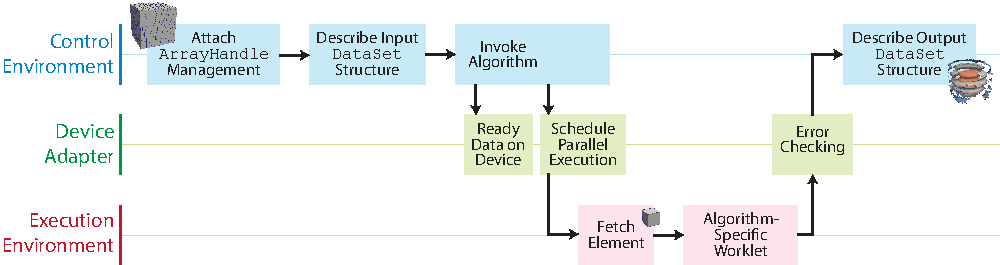
\includegraphics[width=\textwidth]{figures/vtkm-workflow}
  \caption{
    Workflow of an algorithm implemented in VTK-m.
    The ``control environment,'' which runs on a single thread on the host, manages data organization and orchestrates operations.
    The ``execution environment,'' which runs on many threads on the device, performs parallel execution across elements of data.
    A ``device adapter'' manages data movement and control flow between these two environments.
  }
  \label{fig:vtkm-workflow}
\end{figure*}


\section{Introduction}

\ken{Do not add OverLeaf comments to this document. They will not be seen! Instead, use the comment command with your name to add the comment to the text. We'll see the comment when reviewing the paper. The commands are defined near the top of IJHPCASpecialIssue\_VTKm.tex.}

%\ken{Please complete your writing assignments by January 22.}

%\assign{Hank, do an editing pass.}

%The Exascale Computing Project (ECP) brought high-performance computing to the next milestone of capacity computing.\hank{I do not understand the preceding sentence.  Capability?  And we already had HPC.  How did ECP bring HPC?}
As its name would imply, the goal of the Exascale Computing Project (ECP) was to build and make practical the world's first Exascale high performance computers.
Although this goal was nominally to stand up computers capable of a billion billion ($10^{18}$) floating point operations per second, this advancement required a revolution in both hardware and software.
Pivotal to this advancement was the adoption of GPU processors from a variety of vendors as the primary computing engine.
These GPUs provided an unmatched computational throughput relative to the power they consume, albeit at the cost of greater code complexity.

Scientific simulations running on exascale supercomputers can produce data sets of unprecedented
scale, and
visualization and analysis approaches are frequently used to understand the resulting
data and promote discovery.
%
That said, the scale of the data produced by simulations on exascale computers requires
the visualization and analysis approaches to themselves utilize significant computation.
%
Most commonly, this computation is done using the same supercomputer and hardware that produced
the data in the first place.

VTK-m is a software library that \ollie{insert "makes"} it possible to process data sets from exacale computers,
 by implementing classic scientific visualization algorithms redesigned for heavily threaded environments like GPUs.
VTK-m also provides a framework that simplifies the implementation of new algorithms and provides a porting layer to work across multiple processor types.
At the inception of ECP, VTK-m was the byproduct of a research project.
ECP provided the investment to promote VTK-m to production software.
This software that now serves as the underlying visualization implementation across all ECP.
VTK-m is currently used by ParaView, VisIt, and Ascent to execute visualization algorithms on Exascale platforms and others using GPU processing.

This paper provides an overview of the main challenges encountered to make visualization available at the Exascale.
It begins with a brief overview of the VTK-m framework.
It then discuss the largest porting challenges encountered during ECP as the hardware for the final Exascale machines differed dramatically from the pre-Exascale machines.
This is followed by a summary of the performance of VTK-m on the Exascale hardware.
Finally, the paper concludes with a discussion on the software engineering required to integrate VTK-m into usable visualization tools and successes with using VTK-m to solve problems in real science applications.
This includes porting challenges, performance testing and improvement, integration with other ECP software technologies, and the support of ECP applications.

\section{Overview of VTK-m}

\assign{Hank, editting pass (perhaps trimming)}

The origin of the VTK-m library \cite{Moreland2016} is a USDOE ASCR research project to enable scientific visualization on emerging HPC systems.
The main goals of VTK-m are twofold: to serve as a repository for interoperable scientific visualization algorithms well suited to accelerator architectures and to provide a framework that simplifies the development of visualization algorithms that can be ported across many accelerator devices.

\ken{Idea from Jay: summarize the filters and stuff we have done in a table so that people can easily add their work.}

\jay{Table is added and we might simplify this paragraph a little bit and put detailed references into the table.}

At the onset of ECP, VTK-m contained only the most common operations for scientific visualization: contour \cite{Lo2012}, threshold \cite{Maynard2013}, external faces \cite{Lessley2016}, basic surface simplification \cite{Moreland2016}, and rendering \cite{Larsen2015:VR,Larsen2015:RayTrace}.
Although this initial set covers much of the basic needs for scientific visualization, practitioners require much more functionality.
ECP was fundamental in growing this functionality with the introduction of many more algorithms.
Notably, these include clip, connectivity, clean grid, material interface reconstruction, statistics, gradients, density estimation, coordinate transformation, streamlines and other flow algorithms \cite{Pugmire2018}, surface normal generation, mesh quality metrics, resampling, and contour tree \ken{cite} as well as numerous optimizations.
These added features provide the necessary functionality for the tools and applications, discussed later in this paper, that rely on VTK-m to execute on Exascale machines and similar hardware.

VTK-m also internally provides a framework that simplifies the implementation of these and future algorithms as well as ports these algorithms across different devices.
The basic structure of the framework is shown in Figure~\ref{fig:vtkm-framework}.
Code in VTK-m is separated into two separate environments: control and execution.
These correspond to the ``host'' and ``device,'' respectively, in a GPU development environment.
That said, the logical control and execution environments are maintained even when there is not a clear separation between host and device, which is the case for some accelerators such as the Xeon Phi \ken{cite?}.

\begin{figure}[htb]
  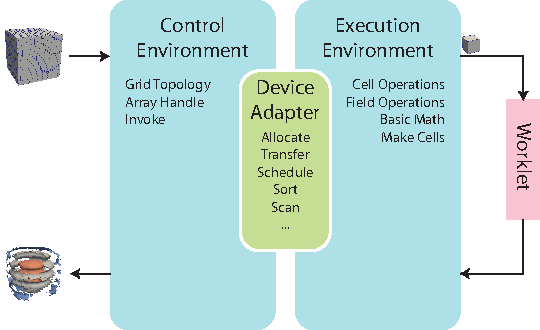
\includegraphics[width=\linewidth]{vtkm-framework}
  \caption{The basic VTK-m framework that allows device portability.}
  \label{fig:vtkm-framework}
\end{figure}

Mesh structures are definined using a flexible data model \cite{Meredith2012} in the control environment.
Based on the structure, the data are divided in small pieces, and the pieces are processed in parallel in the execution environment.

All of these aforementioned structural units are implemented with standard C++14 and are universal for any GPU device.
To achieve portability, VTK-m contains a device adapter that manages interaction with a variety of devices.
The entirety of VTK-m can be ported with a change to the device adapter.

The device adapter enables parallel execution using the data parallel primitive method \cite{Blelloch1990}.
Data parallel primitives allow algorithms to be implemented as a sequence of data parallel operations such as scan, sort, or reduce.
Early work explored how to implement scientific visualization using data parellel primitives \cite{Lo2012}.
To simplify the implementation further, VTK-m provides a layer of meta data parallel primitives \cite{Moreland2021} that are shown to be efficient during use.

\section{Porting Challenges}

Although the pre-Exascale machines gave the VTK-m development team good experience porting to different processor architectures, the design of the Exascale machines Frontier and Aurora introduced new technical challenges.
This section reports the most major modifications of VTK-m to make it feasible to run on the Exascale hardware.

\ken{
  Each subsection should be roughly 1/3 page.
  (1 + 1/3 page total.)
  The subsection should start with a paragraph defining the problem/motivation.
  The following paragraph should give an overview of the approach.
  The remaining paragraphs can go into technical challenges that were encountered and how they were addressed.
}

\subsection{Adopting Kokkos}

\assign{Sujin}

\begin{figure}[htb]
  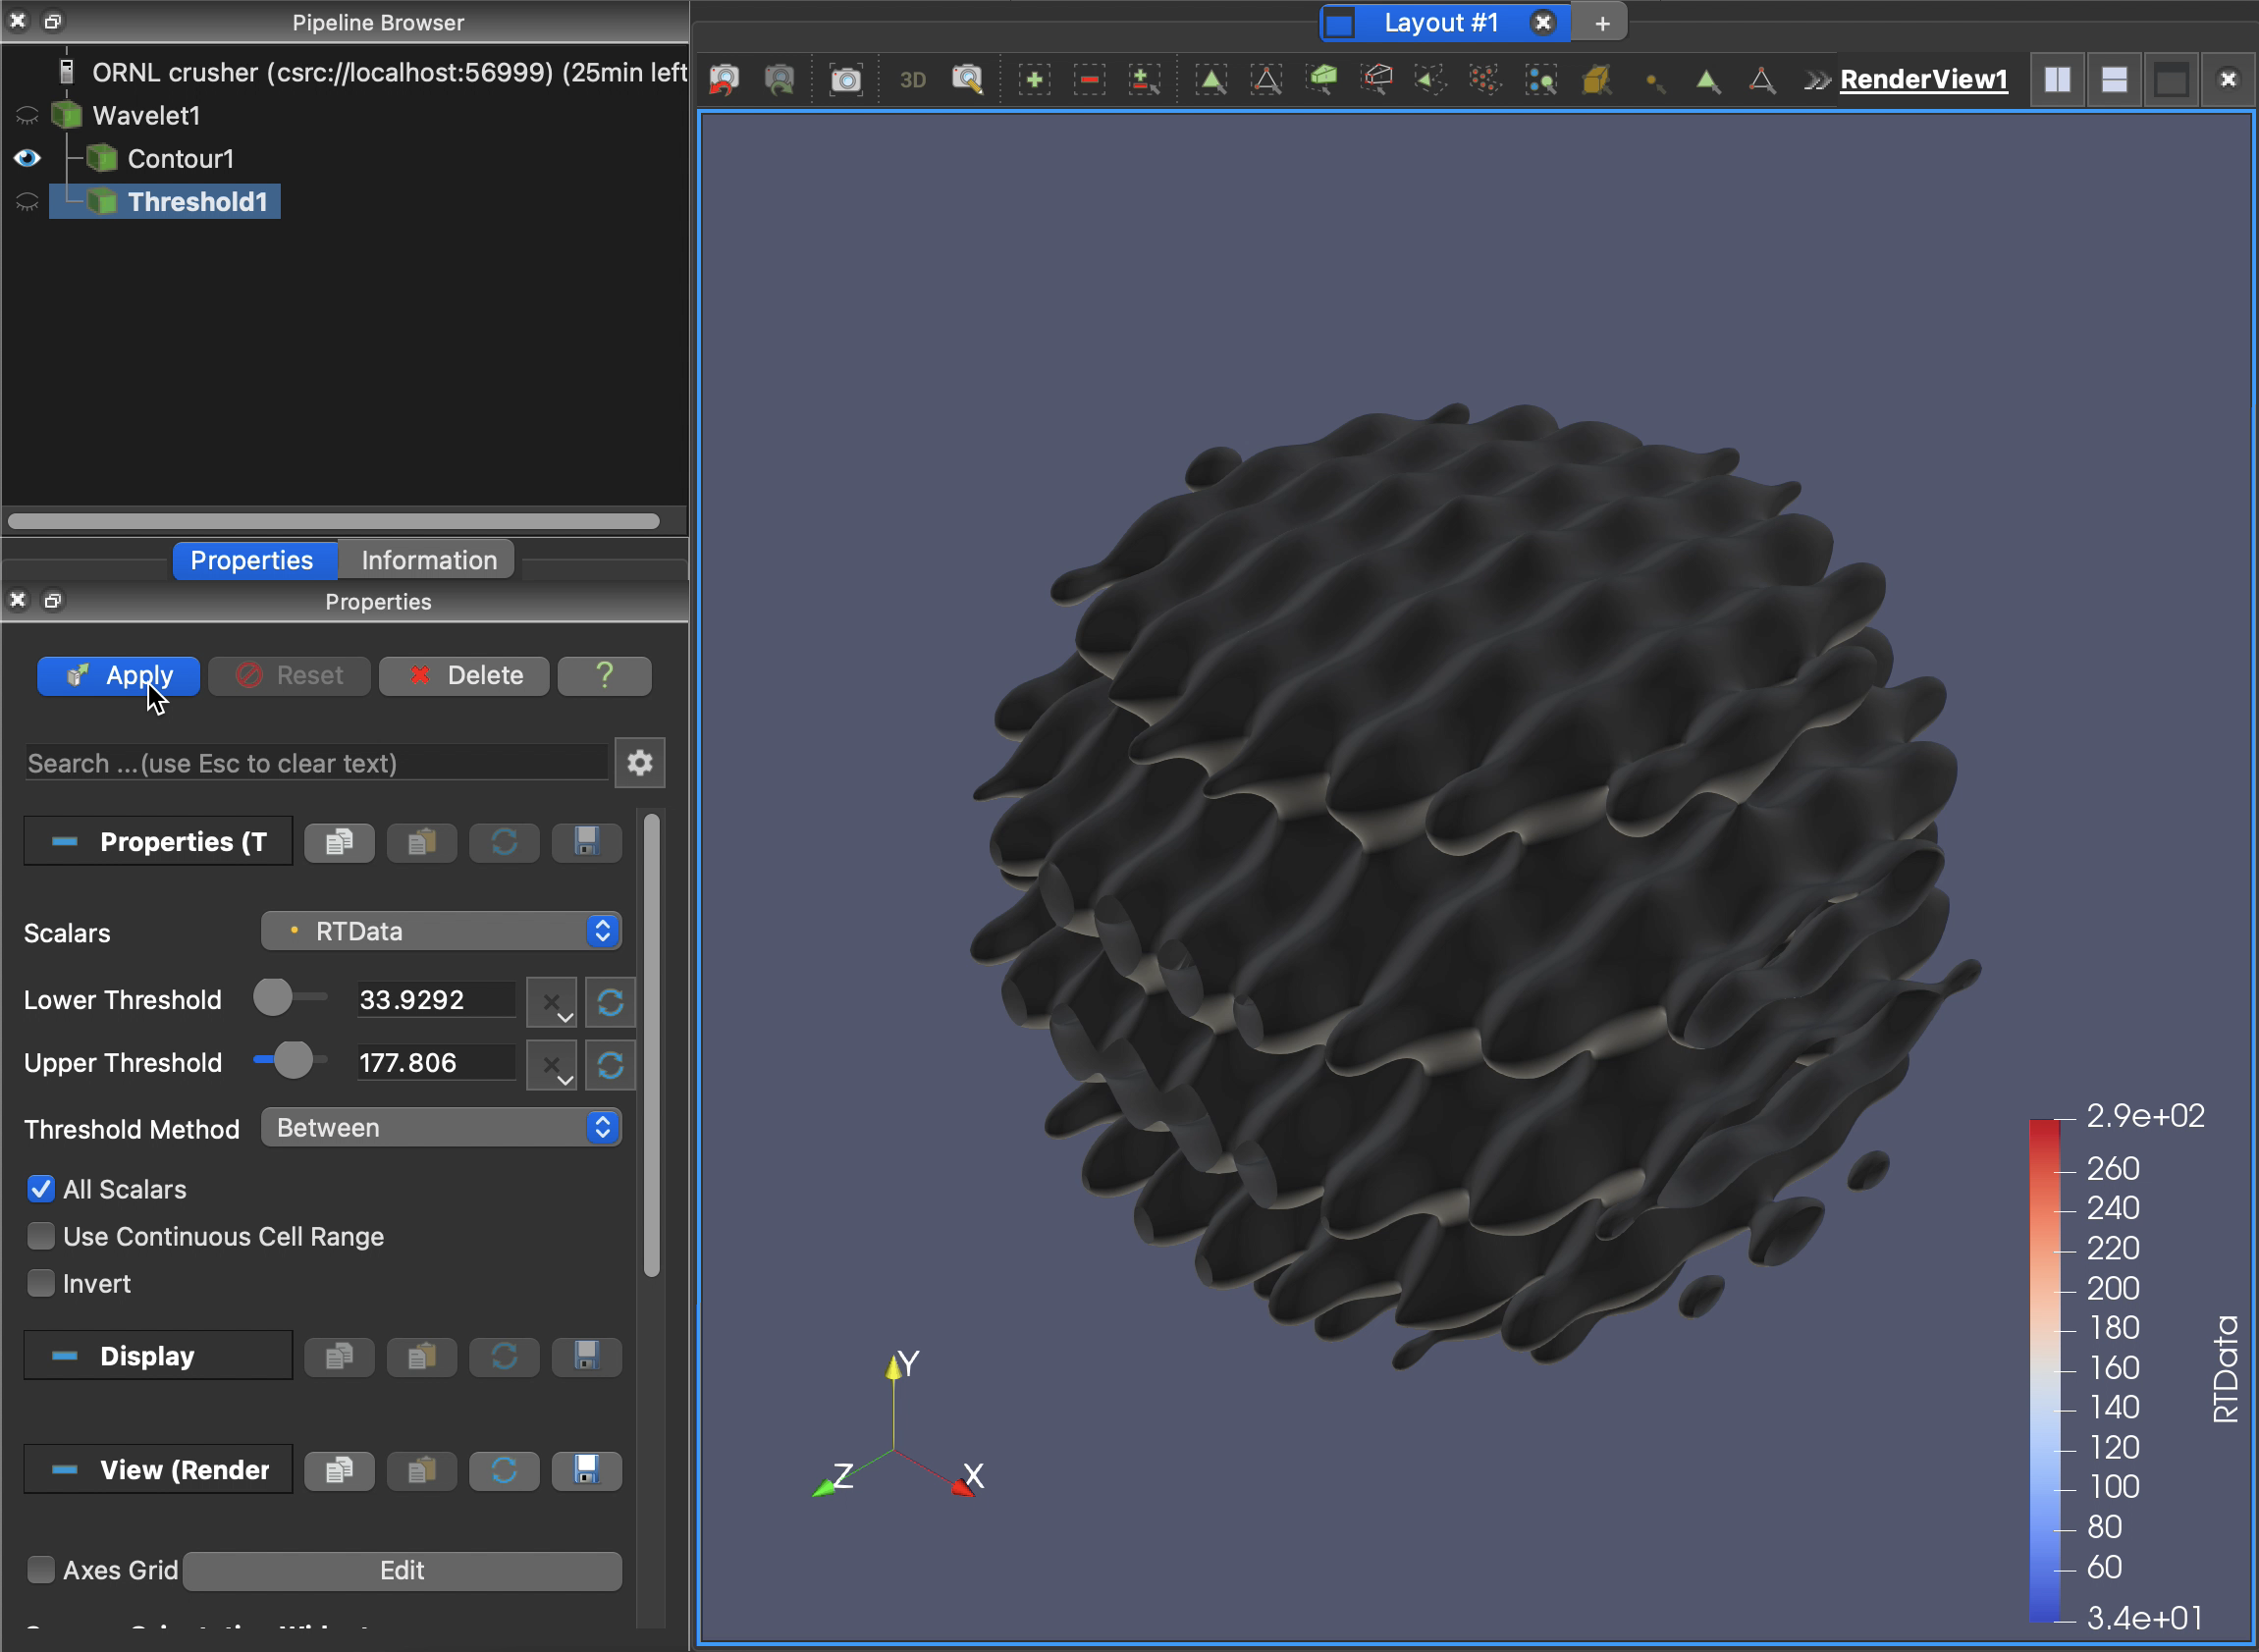
\includegraphics[width=\linewidth]{figures/paraview-crusher.png}
  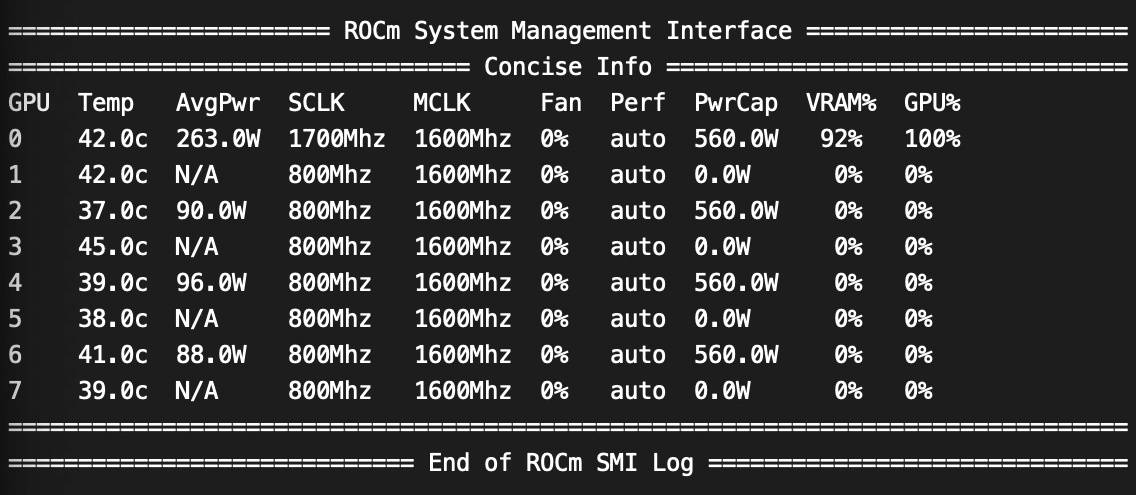
\includegraphics[width=\linewidth]{figures/threshold-vtkm-gpu-usage-crusher-small.png}
  \caption{
    ParaView, with integrated VTK-m accelerated filters, running on Crusher.
    VTK-m is using the Kokkos device adapter.
    The output of rocm-smi command is being used to verify and monitor GPU usage by the filters.
    \ken{I think it would be better to move this figure (or something like it) to the ParaView section.}
  }
  \label{fig:paraview-crusher}
\end{figure}

%\sujin{
%The first two paragraphs can be simplified by referring to the device adapter explanation in the VTK-m overview section
%}
As described in the overview of VTK-m,
one of the main features that VTK-m supports is ``write once, compile anywhere'' for its algorithms.
%VTK-m filter’s are implemented in modern C++. The build system of VTK-m can then compile these for one or more of the various parallel devices that it supports. This level of compatibility is achieved through the use of an abstraction layer in VTK-m called the \texttt{DeviceAdapter}.
A device portability layer called a device adapter allows algorithms written with standard C++ features run across all devices.
These device adapters wrap a parallel execution capable device and provide functionalities for parallel-task scheduling, memory management, and several commonly used parallel algorithms like sort, reduce, etc, through a common interface.
These are implemented on top of the native libraries used to program these devices.
%At the most basic level, a device adapter only needs to provide support for memory management on the device, a way to execute an n-way, fine-grained, parallel task on the device, and atomic operations.
%There are generic implementations for all of the parallel algorithms like sort, reduce, scan, etc, but it is possible to override these with specialized implementations for best performance.
%The early versions of VTK-m had \texttt{DeviceAdapter} implementations for single threaded CPUs using standard C++, multithreaded CPUs using the threading building blocks library or OpenMP, and GPGPUs using CUDA.

When the architectures for the initial two major Exascale machines, Aurora and Frontier, were announced, it was revealed that they would be using two completely new GPGPU architectures, with their own native libraries (SYCL and HIP).
This would have required additional two new device adapter backends.
Although the device adapter layer greatly simplifies the porting of VTK-m code, implementing device adapters themselves is not trivial.
So, although it would be technically feasible to design device adapters for two new devices, it would have required significant effort.
%Maintaining these backends together with the already existing backends was would require a lot of effort, especially for a project that is primarily concerned with implementing highly parallel visualization algorithms.

For these reasons, we looked towards another ECP project called Kokkos~\cite{Edwards2014, Trott2022}. Kokkos is a library for implementing performance portable applications in C++. Similar to VTK-m, Kokkos also supports multiple device backends, including HIP and SYCL used by the Exascale systems. So, with just one device adapter built on top of Kokkos, we are able to target both the machines.
This allows us to write the VTK-m device adapter once to the Kokkos API and defer the work of interfacing with the different ECP device APIs to the Kokkos team, who were already doing this for other ECP projects.

\ken{Is there anything more to be said about the interface? Was there anything particularly challenging? Any mismatch between the APIs? Any ``hacks'' that might have happened?}


\subsection{Addition and then Removal of Virtual Methods}
\label{sec:virtual-methods}

\assign{Ken}

Ideally, an algorithm
%that operates on arrays
will know the data types that it will operate on.
Unfortunately, this is seldom the case for VTK-m where data ingested from different sources can have any number of basic types
%(32- or 64-bit floats or fixed precision values encoded in integers)
and different types of memory layout.
In the early years of ECP, this problem was addressed by compiling algorithms in VTK-m for all possible types that could be encountered.
However, the amount of potential cases generated is too large to be practical.

C++ objects with virtual methods are a natural solution to this problem, and as they became available on CUDA devices, VTK-m started using virtual methods to hide the structure of arrays.
This originally addressed some of the issues with type abstraction.
However, this solution worked poorly and was later abandoned for two reasons.
First, using virtual methods introduced problems with library linking as the compilers had to collect any possible code that might be needed to be loaded on the device.
Second, when ECP announced that its Exascale machines would be using GPUs other than CUDA, it was unclear how well they would support virtual methods or even if they would be supported at all.

Consequently, the VTK-m development team pivoted.
Virtual methods were removed from the VTK-m code that ran on devices.
To manage the operations on types without using virtual methods, VTK-m employed a trio of strategies: multiplexing the type in the algorithm, generalizing the stride in arrays, and providing fallbacks when unexpected types were encountered.

The first strategy, multiplexing, required the use of a type agnostic storage object.
For this, a \texttt{Variant} class was added to VTK-m.
The \texttt{Variant} takes a list of types as template parameters, and it can hold exactly one of these objects at a time.
At runtime, the proper type can be queried and extracted.
%Implementing the \texttt{Variant} to avoid type punning across all device compilers was challenging.
Although multiplexing from a variant object still requires separate compilation for all possible types, it limits the code that must be recompiled to make it more manageable.

The second strategy required a redesign of the array management in VTK-m.
Where the original design of array management completely abstracted the implementation, the new design based array management on known buffers of memory.
This in turn provided a way to generalize the representation of an array component by defining a stride in the buffer.
In this way, an algorithm no longer had to be compiled for a specific data layout.
It could instead apply a stride to the array and use any layout.

The third strategy recognized that although a great number of types are possible, many are rarely if ever encountered in practice.
Therefore, instead of attempting to compile a function for any possible type, it is possible to instead compile for the most likely types and then have a fallback for the cases when the type is unexpected.
The typical solution is to copy the array of unknown type to an array of a known type.
This feature was included into the filter interface overhaul, which is described in the next section.

\subsection{Filter Interface Overhaul}

\assign{Ollie}

The majority of algorithms in VTK-m are contained in what is called a ``filter'' object.
A filter takes a data set, performs some operations to modify it, and returns the resulting data set.
Filters provide the outwardly facing API to processing data in VTK-m.
However, as previously described, these data sets can have any number of data types and structures.
The VTK-m filter base class needs to provide a mechanism to resolve data types.
That is, the filter base class needs a way to call a templated method in a derived implementation class with fully resolved data types.

Since a C++ template method can not also be a virtual function, which is needed for typical runtime polymorphism, the original design used a rather complicated technique called the curiously recurring template pattern (CRTP) \cite{Coplien1995} to emulate it.
CRTP works by making the type of the derived class a template argument to the base class.
When the base class needs to call a method in the derived class, rather than use a virtual method it recasts itself as the derived class and calls the method directly.
This allows the base class to iterate through a list of supported data types and call a templated method in the derived class to implement the algorithm on each one.

%The addition of \texttt{Variant} and the redesign of array management in VTK-m also enabled us to further redesign the developer's interface for \texttt{Filter}s.
%Previously, a filter implementation had to provide a \texttt{DoExecute} method that took a template \texttt{ArrayHandle<T>} as one of its arguments.
%Filter base classes would iterate through a list of supported data types, defined by the filter developer, instantiate and call \texttt{DoExecute} with each of the concrete type \texttt{T}.
%There were several downsides of this design.
%First, as mentioned above, we had to instantiate a large number of \textit{DoExecute}, one for each of \texttt{T} in the list.
%Second, since a C++ template method can not also be a virtual function which is needed for runtime polymorphism, the original design used a rather complicated technique called \emph{Couriously recurring template pattern (CRTP)} to emulate it.

However, using CRTP also made the base filter class itself a class template, and its execution methods required exposed definitions that needed to be recompiled at every instance of its use.
This made the VTK-m filter library essentially a header-only library, and clients using it had to include all the necessary implementation in the header files.
When compiling client code, all those header files had to be parsed and classes and methods had to be instantiated.
As a consequence, it took a long time to compile applications of VTK-m.
This issue was most prominent when compiling for GPU devices since most device compilers were not as efficient in handling C++ templates as host compilers.
When integrated as part of an in situ pipeline, simulation code calling VTK-m's filters also needed to be compiled by a device compiler, thus exacerbating the problem.
In some extreme cases, the whole compilation process took more than 24 hours to complete.

The new design turned this type dispatching mechanism around.
The responsibility of type dispatching was shifted from the filter base class to the derived implementation classes.
The execution method in the derived class is no longer a template; it accepts a data set containing ambiguous types.
This increases the burden on the algorithm developers who now have to resolve types themselves.
To compensate, VTK-m provides an alternate dispatching mechanism by providing various forms of a ``cast-and-call'' mechanism on the data set's elements.
The derived filter performs the type dispatching by passing a data set element to a cast-and-call along with a templated, callable object.
This callable object is generally the type dependent, core business logic of the filter implementation wrapped inside of a C++14 generic lambda expression.
The lambda expression will be instantiated with types from a pre-defined type list by the cast-and call mechanism.

The cast-and-call will attempt to resolve the data to a prescribed list of types.
When the type of the data is not part of the type list, the cast-and-call can fallback to a known type as described in the previous \nameref{sec:virtual-methods} section.
The pre-defined type list and fallback limit the number of instantiations of the lambda expression.
Using cast-and-call with lambda expressions in this way also limits the portion of code to be instantiated.
In contrast, the original design required the whole body of the filter implementation to be instantiated.

Since the filter execution methods are no longer template methods, they can be virtual methods.
Note that the filter methods in question are explicitly run in VTK-m's control environment, which means they will only be run on the CPU host of the machine.
Previously discussed issues with virtual methods on GPUs do not apply here, so creating virtual methods here is not problematic.
The virtual methods eliminate the need to use the CRTP technique.
As a consequence, the whole filter class hierarchy has became non-template classes as well.
The library is no longer a header-only library and can be built as a traditional, pre-compiled library.
The filter library is further divided into several modules with each separately compiled into a \texttt{.so} file.
Applications now do not need to be compiled by a device compiler simply because they are using VTK-m.

The ability to control template instantiation and separate, concurrent compilation of the filter library has greatly reduced application build time because they no longer has to compile many VTK-m templates.
Rather, applications simply link to methods in the VTK-m library.
We have also found that the new approach provides other compile-time saving opportunities within the library.
For example, some filters incorporate the functionality of others as a subprocess.
The new filter structure allows filters to be compiled once and have their functionality leveraged by other filters.
For example, the compilation of VTK-m's material interface reconstruction filter was reduced by a factor of 9 by linking to the mesh quality filter rather than recompiling it.
The new filter structure also enables dividing the code into multiple translation units (i.e. separate C++ source files).
Although this does not necessarily reduce the aggregate compile times, it more effectively leverages cores in parallel builds and reduces the possibility of compiler crashes from running out of resources.
%\ollie{Ken can you add some concrete timing measure as you did before here?}
%\ken{I will look. I probably don't have anything concrete. I'm not sure I captured enough data to measure the time before the filter change and the time after. (A lot changed in the interim anyway.) But I think I can pull up a couple of examples.}

\subsection{GPU-to-GPU Transfers}

Modern HPC GPUs allow direct GPU-to-GPU communication. This provides GPUs with an efficient mechanism to directly send data stored in their device memory to the target GPU device memory. This contrasts with the traditional and costly GPU communication pattern that consists in first copying the desired data from the device memory to host memory, transferring it, and then again copying the received data from host memory to device memory.

Enabling this feature in VTK-m required changes in the source code of both VTK-m itself and DIY, a third-party library that VTK-m uses to manage its MPI communication~\cite{Peterka2011,Morozov2016}.
%The reason for making changes to DIY is that VTK-m delegates data marshaling and remote communication through the DIY library.

The DIY library changes consisted of adding routines that allow sending and receiving raw pointers directly encapsulated in a newly introduced ``blob'' data type. This contrasts with the regular operation of DIY that copies and serializes data before sending and receiving. In addition to that, we have also introduced a new API in DIY that controls the ownership of the passed raw pointer.

The corresponding VTK-m changes consisted of modifying the VTK-m class that manages memory buffers and their location among host and devices.
In particular, the changes overwrite the DIY serialization to directly pass these memory buffers to and from DIY.
Additionally, a new CMake option named \texttt{VTKm\_ENABLE\_GPU\_MPI} that activates direct GPU-to-GPU communication of VTK-m buffer objects was added.
This in turn, enables direct GPU communication in VTK-m since most of the VTK-m storage entities are composed of VTK-m buffers. 

The main challenge found during the implementation of this feature was maintaining compatibility with the Frontier target system.
The problem was that the software stack in the target system was a moving target with frequent updates that in many cases required us to modify build and runtime parameters and, in some other cases, perform changes to the VTK-m and DIY source code.
This challenge was minimized by provisioning the VTK-m Gitlab project with nightly jobs that build and run tests using this feature in the Frontier test-bed system.
This allowed us to quickly identify problems arising in changes to either VTK-m's source code or the Frontier software stack.

\section{Performance on Exascale Hardware}

\subsection{Frontier}

\subsection{Aurora}

\section{Integration into Visualization Tools}

Throughout the life of the ECP, the \vtkm team collaborated heavily with other ECP software technology teams.
The scope of the \vtkm project was to provide the fundamental technology to run scientific visualization algorithms on GPUs, which account for the vast majority of the computational power of current exascale machines.
Other ECP teams, most notably the ALPINE project, developed tools that would leverage \vtkm while directly addressing application needs.
This arrangement avoided the redundant work of multiple teams developing their own visualization solutions and prevented users from having to use yet another software interface.
In this section, we discuss the major visualization tools that we integrated \vtkm with.

%% \ken{
%%   Each subsection should be roughly 1/2 page plus have an image demonstrating the tool with \vtkm that is about 1/3 page.
%%   (3 + 1/3 page total.)
%%   The subsection should start with a description of the tool.
%%   (Exception: the last subsection starts with a description of the lengthy process from committing code in \vtkm to it being available in a tool.)
%%   The following paragraphs describe how \vtkm is integrated at a high level.
%%   Avoid details like classnames.
%% }

\subsection{ParaView}

%\assign{Sujin}
The \vtkm library provides high-performance implementations of several visualization algorithms for highly parallel processors.
However, features such as file I/O, rendering, and pipeline management, which are all essential parts of a full-featured visualization toolkit, are beyond the scope of \vtkm.
On the other hand, ParaView is a mature visualization software that has robust implementations of these features.
Therefore, we wanted to integrate \vtkm into ParaView in such a way that ParaView can use \vtkm filters to accelerate its operations when a \vtkm implementation and hardware that concurrently executes many threads is available.

We also wanted the \vtkm accelerated filters to be as easy to use as possible.
Therefore, we chose to integrate \vtkm using VTK and ParaView's factory-instantiation feature.
Because ParaView is implemented on top of VTK and internally relies on VTK filters, both VTK and ParaView will be mentioned interchangeably in this section.
Filters in ParaView are instantiated via a factory method.
There can be multiple implementations available for a filter, and the factory method chooses an appropriate implementation at run time based on given criteria.
With this method, we can override the default ParaView filters with \vtkm-based filters.
Currently, \vtkm accelerated filters that override traditional CPU implementations are available for some commonly used filters such as contour, threshold, and gradient.
%Adding overrides for more filters is a straightforward process as discussed in the following paragraphs.
Additional \vtkm filters can be added by providing additional overrides.

To override a ParaView filter, we first need to implement a \vtkm wrapper filter in VTK to provide the interface of the base VTK/ParaView filter and use \vtkm filters and routines for its operation. The following steps provide a high-level overview of how a \vtkm wrapper filter is implemented in VTK/ParaView:
\begin{enumerate}
    \item Check the filter parameters and only proceed with \vtkm processing for configurations supported by the \vtkm filter implementation.
    \item Convert the input VTK datasets to \vtkm datasets. 
    \item Execute the \vtkm filter on the data.
    \item Convert the output of the \vtkm filter back to VTK datasets.
    \item If an error occurs at any point during the above steps, then fall back to the default VTK implementation. Errors in \vtkm are typically signaled via C++ exceptions.
\end{enumerate}

For the dataset conversion from VTK to \vtkm and back, we implemented several helper routines. These are zero-copy operations for most cases because, whenever possible, only the ownership of the pointers to the underlying resources is transferred. Even copies from host-to-device and device-to-host are minimized by using a \vtkm dataset wrapper in VTK called \texttt{vtkmDataSet}, which implements the \texttt{vtkDataSet} interface and only copies the data when required. Another commonly used ParaView functionality is computing the range of the various fields of a dataset. This has also been accelerated by using \vtkm, which speeds up the computation and avoids memory transfer from device to host.

\begin{figure}[t]
  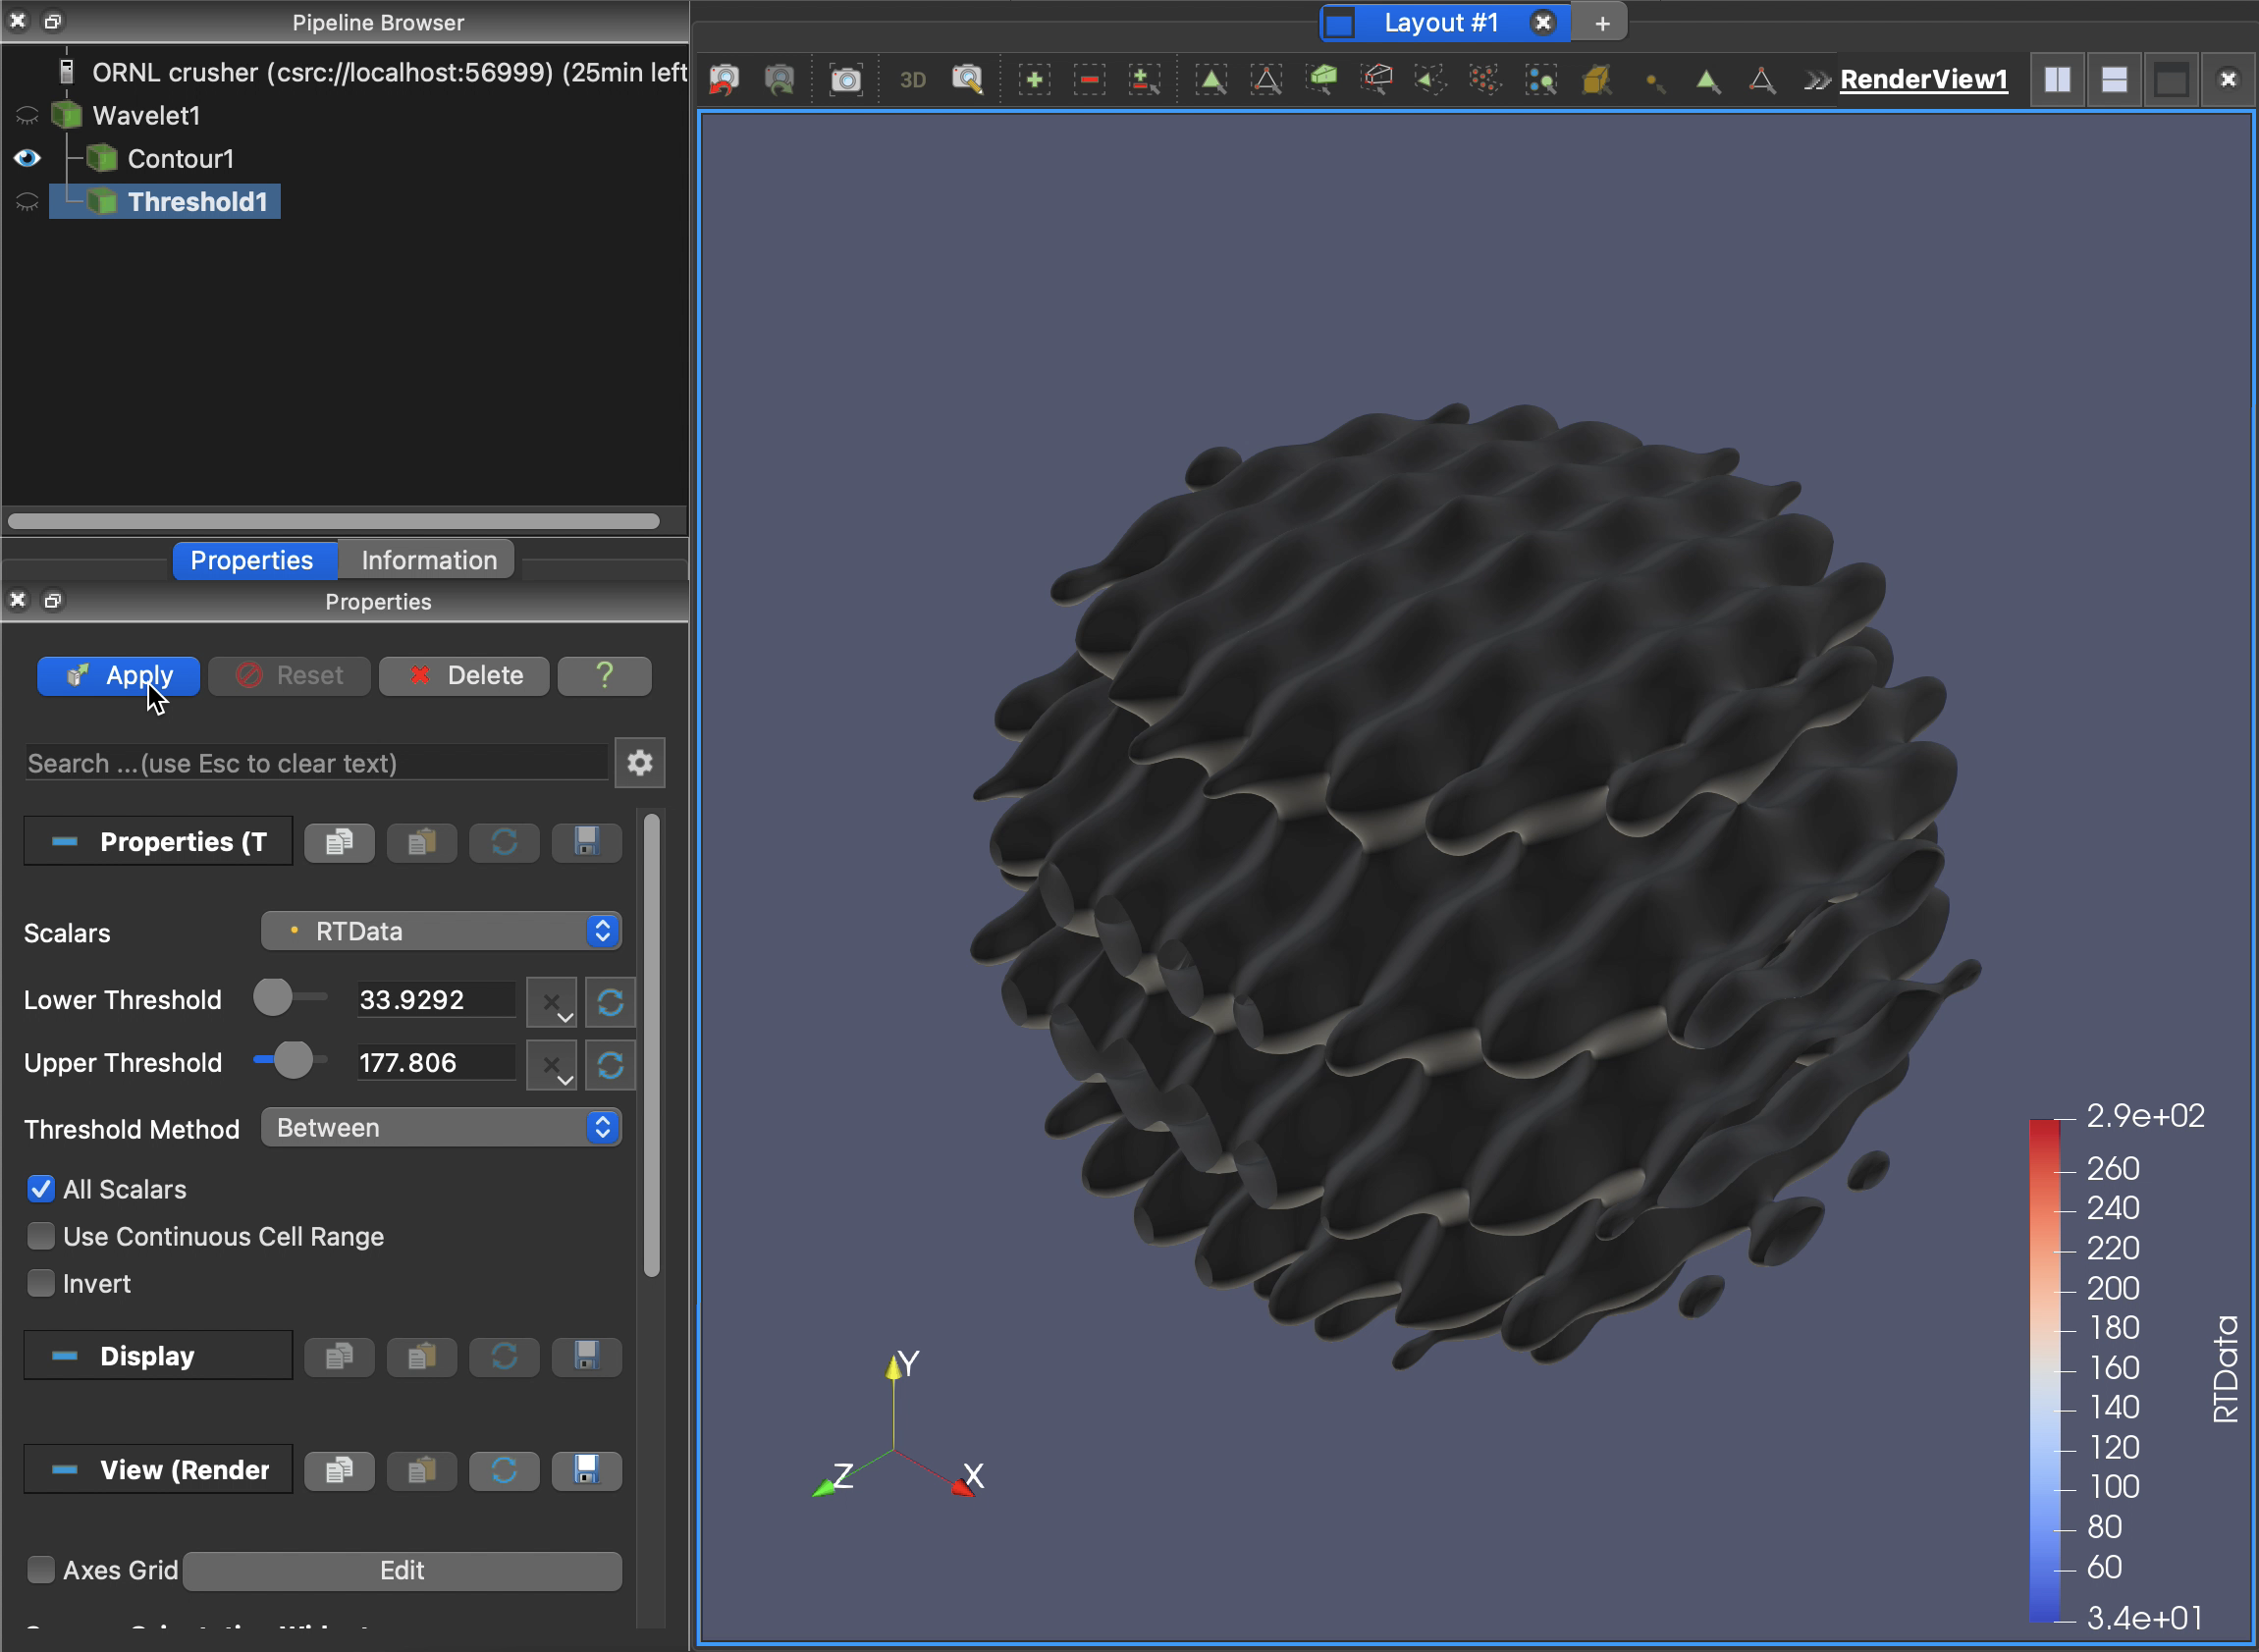
\includegraphics[width=\linewidth]{figures/paraview-crusher.png}
  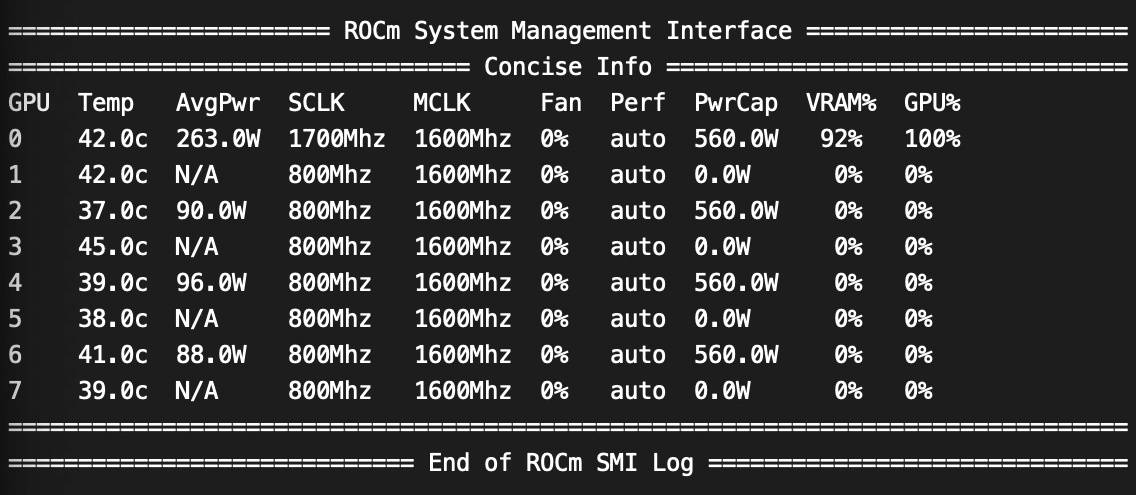
\includegraphics[width=\linewidth]{figures/threshold-vtkm-gpu-usage-crusher-small.png}
  \caption{
    ParaView with integrated \vtkm accelerated filters running on Crusher, an early access test bed for the Frontier system.
    \vtkm is using the Kokkos device adapter.
    The output of the \texttt{rocm-smi} command is being used to verify and monitor GPU usage by the filters.
    %\ken{I think it would be better to move this figure (or something like it) to the ParaView section.}
  }
  \label{fig:paraview-crusher}
\end{figure}

Figure~\ref{fig:paraview-crusher} shows an example of ParaView running with \vtkm accelerated filters on Crusher, which is an early access test bed for the Frontier system.
As described in the \nameref{sec:adopting-kokkos} section, \vtkm is using the Kokkos device adapter on this hardware.
The bottom of the image shows the output of the \texttt{rocm-smi} command, which is used to verify and monitor the GPU usage by the filters.

\begin{figure}[htb]
  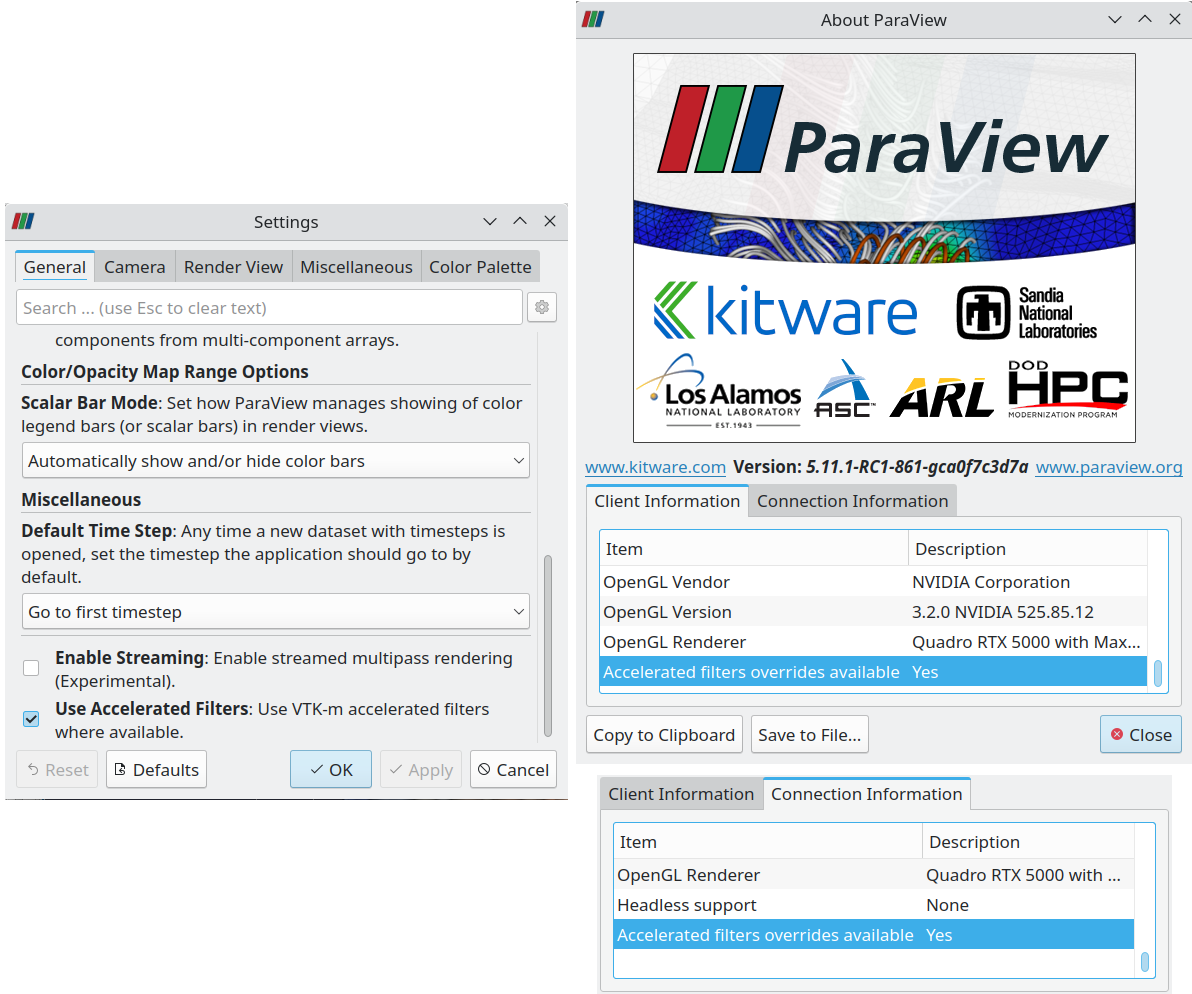
\includegraphics[width=\linewidth]{figures/pv-override-settings.png}
  \caption{
    Left: The \texttt{Use Accelerated Filters} ParaView setting can be used to activate or deactivate accelerated filter overrides at run time.
    This setting is shown regardless of whether or not ParaView was built with the override support.
    Right: The availability of the accelerated filter overrides on clients and servers can be found in the \texttt{About ParaView} dialog box.
  }
  \label{fig:paraview_settings}
\end{figure}

%\ken{This last paragraph might be more detail than needed.}
% The wrapper filter needs to be registered with the factory for the factory instantiation to work. This is done at the build configuration using the CMake function:
% \texttt{\_vtkm\_add\_override("vtkBaseFilter" "vtkmAcceleratedFilter")} Then, the accelerated filters need to be enabled using the CMake option \texttt{VTK\_ENABLE\_VTKM\_OVERRIDES}. They can also be turned on or off during run time through ParaView settings as shown in Figure~\ref{fig:paraview_settings}.
%\sujin{Ken, please review if the changes are satisfactory}
\vtkm accelerated filter overrides are available in recent releases of ParaView and can be enabled during building.
If enabled, the overrides can also be turned on or off at run time using the ParaView settings (Figure~\ref{fig:paraview_settings}).

\subsection{VisIt}

%\assign{Eric}
VisIt is a scientific visualization and analysis tool that operates on mesh-based field data.
Its functionality is grouped into four major categories: plots, operators, expressions, and queries.
All four of these capabilities are built on a filter infrastructure that operates on mesh-based fields.
Plots are somewhat special in that they consist of a rendering capability that may include some built-in filter operations.
To date, the \vtkm integration has consisted of modifying the filter infrastructure to use \vtkm filters when comparable \vtkm functionality exists.
%There has not yet been an effort to utilize \vtkm's rendering capabilities.


Previously, VisIt's filters used VTK filters and VTK datasets.
The filters were enhanced to support using both VTK and \vtkm.
When \vtkm is enabled in VisIt and the filter supports \vtkm, the filter will use \vtkm.
The internal dataset representation was also modified to support providing either a VTK dataset or a \vtkm dataset.
When the filter is set to use VTK, it will request the data as a VTK dataset or convert the dataset to a VTK dataset if it is stored as \vtkm.
Conversely, when the filter is set to use \vtkm, it will request the data as a \vtkm dataset and convert it if necessary.
It will use zero-copy conversions whenever possible.

\begin{figure}[htb]
  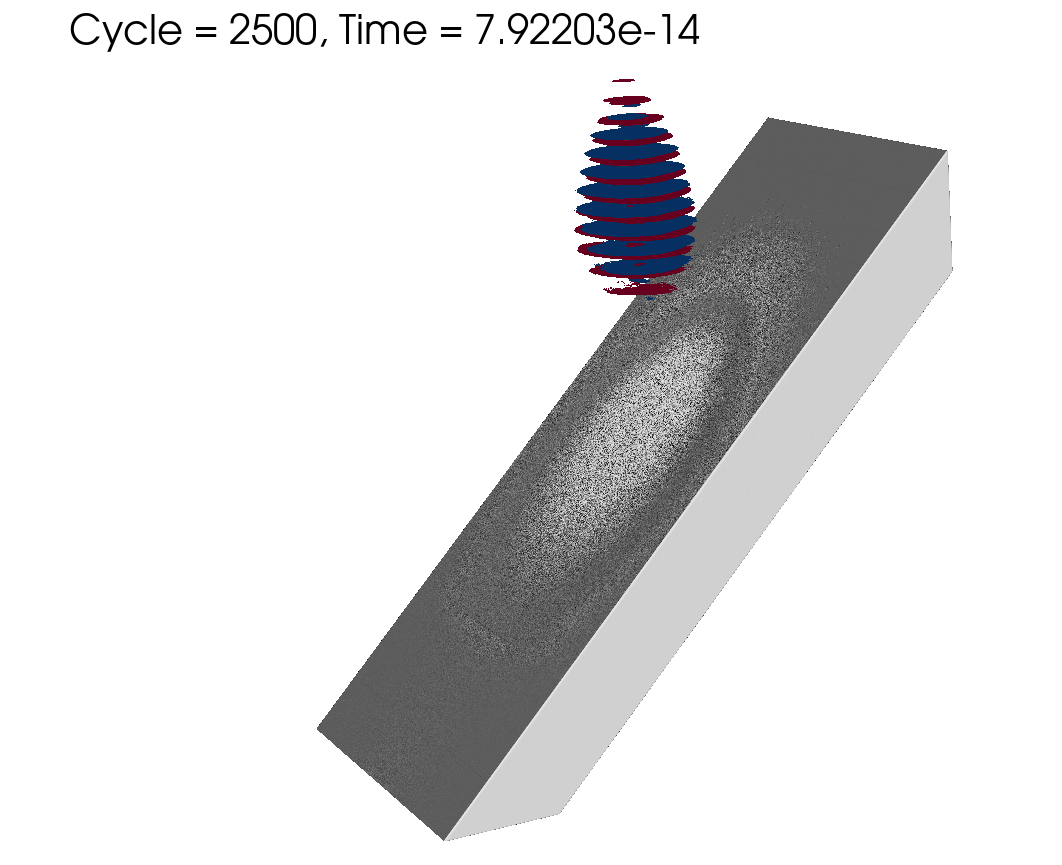
\includegraphics[width=\linewidth]{figures/visit_warpx_frontier.png}
  \caption{Visualization from a 70-billion cell WarpX simulation and Gordon Bell submission~\citep{FedeliHuebl2022} visualized with 2,048 GCDs on Frontier using VisIt.}
  \label{fig:visit_warpx_frontier}
\end{figure}

Figure~\ref{fig:visit_warpx_frontier} is an image generated by VisIt running on Frontier and using 2,048 GCDs across 256 nodes.
The surfaces were generated by using the \vtkm contour filter and were rendered in parallel by using Mesa 3D.
\vtkm is using the Kokkos device adapter for AMD GPUs.

\subsection{Ascent}

%\assign{Nicole}
Ascent is a lightweight, in-situ visualization and analysis library designed for running multiphysics simulations on HPC systems. As an in-situ library as opposed to a post-hoc visualization tool, Ascent shares execution resources with the simulation and can process the data as it is generated, thereby reducing I/O costs, although it must pause the simulation to do so. To minimize the encumbrance on the simulation and execution resources, Ascent's lightweight design ensures a smaller memory requirement. It is written using efficient distributed-memory and many-core libraries to guarantee performance and scalability on current and next-generation HPC platforms. Ascent has three main use cases: creating pictures, transforming data, and capturing data. Ascent is easy to use with only five API calls; supported in C, C++, Python, and Fortran; and provides an infrastructure to integrate custom analysis.
The data interface between simulation code and Ascent is managed through the Conduit API~\citep{Harrison2022}, which provides a simplified interface for passing data and describing structure.

Although optional, \vtkm is a dependency for Ascent because it is currently the only option for rendering low-order mesh data and provides filters for transforming and/or analyzing the simulation data (e.g.,
slice, histogram, contour).
Ascent also leverages \vtkm's zero-copy capabilities as well as its ability to pass device-pointers; these features allow the simulation data to remain on the device and be passed directly to Ascent and then on to \vtkm without being transferred to host memory.
\vtkm has been integrated into Ascent via a (previously external) library called VTK-h (VTK hybrid) that combines \vtkm's shared-memory, high-performance filters with MPI's efficient distributed-memory coordination.

Figures~\ref{fig:warpx_highres} and~\ref{fig:warpx_lowres} show in-situ renderings of the WarpX simulation (see the \nameref{sec:warpx} section later in this paper) generated by Ascent and executed on the OLCF's exascale supercomputer, Frontier.
The simulation was executed at two resolutions: 578.8 million cells across 552 GCDs on 69 nodes and 4.63 billion cells across 4,416 GCDs on 552 nodes.
Ascent used \vtkm filters to upscale the data along multiple axes, generate isosurfaces, and clip several fields before using \vtkm's raytracer and volume renderer to generate the final images.
To guarantee performance, \vtkm uses the Kokkos device adapter for AMD GPUs. 

%\begin{figure}[htb]
%  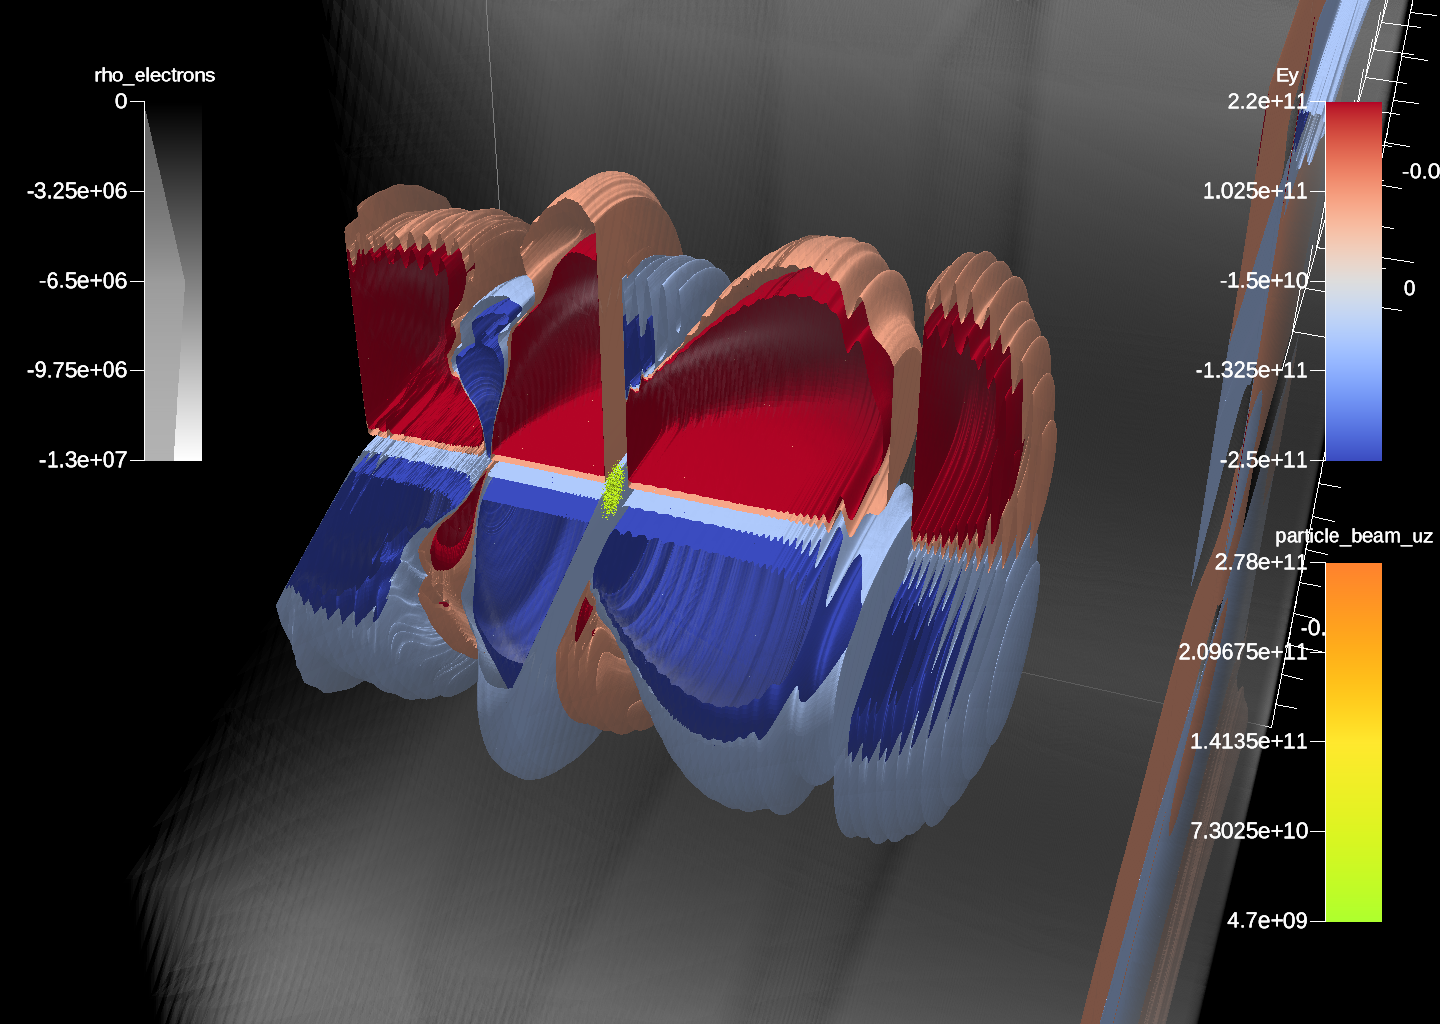
\includegraphics[width=\linewidth]{figures/warpx_stages_lwfa.png}
%  \caption{WarpX in situ visualization of a laser-wakefield accelerator on 552 nodes containing 4,416 GPUs on Frontier using Ascent and \vtkm.
%  The inset shows an early simulation time step at high resolution.}
%  \label{fig:warpx_lwfa}
%\end{figure}

\subsection{Alternative Delivery Mechanisms}

%\assign{Tushar}

Integrating a new feature that was implemented with \vtkm filters into visualization software such as ParaView or VisIt can be a lengthy process.
For example, making a \vtkm filter available in ParaView requires multiple steps, including implementing a VTK filter that wraps the \vtkm filter, completing the arduous process of contributing the change to the VTK project, and then repeating similar steps in ParaView itself.
Such time-consuming software integration can hinder the availability of \vtkm filters inside visualization tools and limit the opportunities for \vtkm filters to increase the pace of scientific discovery.

Our ultimate goal is to make \vtkm filters practical for real use and to put tools in the hands of end users in a timely manner.
An alternative approach to a full integration through the visualization software stack is to provide this functionality through a plug-in that is supported by tools such as ParaView and VisIt.
For the plug-in approach, the \vtkm filter is still wrapped inside a VTK filter, but the time needed for the software integration and testing in VTK and ParaView can be bypassed.

Figure~\ref{fig:uncertainty-plugin} illustrates the \vtkm isosurface uncertainty filter~\citep{Wang2023, Athawale21} made available in ParaView via the plug-in method. The isosurface uncertainty filter is one of the major successes of the \vtkm library because it is the first production-level uncertainty visualization filter deployed for efficient large-data analysis. Using the plug-in method depicted in Figure~\ref{fig:uncertainty-plugin}, \vtkm filters can be easily combined with existing filters in ParaView for improved data comprehension.

\begin{figure}[htb]
  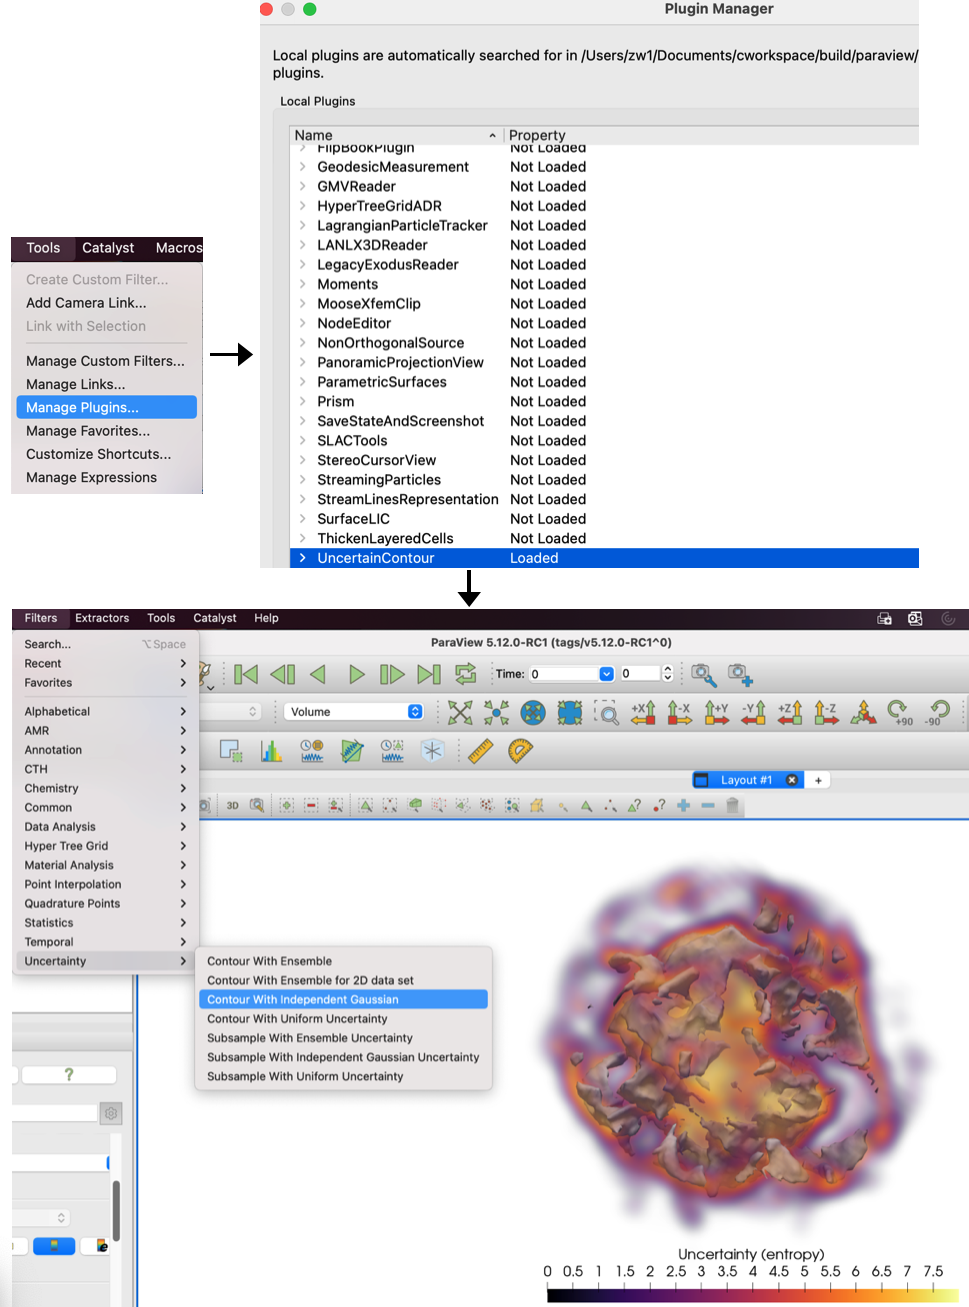
\includegraphics[width=\linewidth]{figures/isosurfaceUncertaintyPlugin.png}
  \caption{Integration of the \vtkm isosurface uncertainty filter in ParaView using the plug-in approach for visualization of large-scale supernova simulations~\citep{Sandoval2021}.}
  \label{fig:uncertainty-plugin}
\end{figure}



%% \ken{
%%   Talk about how you can deliver new functionality to these tools outside of the pipeline of implement in \vtkm $\rightarrow$ VTK $\rightarrow$ Tool.
%%   Use uncertainty plugin as an example of doing this.
%% }

\section{Interfacing with Applications}

The ultimate goal of the \vtkm work for the ECP was to provide scientists with the tools needed to understand large amounts of data and make scientific discoveries.
The previous sections of this paper describe the efforts for making these tools available.
This section provides some examples of applying \vtkm and its companion enabling technologies to real-world science problems, which often happens through the visualization tools described in the previous section.

%% \ken{
%%   Each subsection should be up to 2/3 pages plus have images up to 1/2 page.
%%   (3.5 pages total.)
%%   The section should start with a layperson overview of what the domain problem is, what scientists are doing to study the problem.
%%   The section should then explain how visualization fits in to help.
%%   Explain the technical solution of how \vtkm was integrated into the system and describe the final result.
%%   The section may repeat for multiple things that were done.
%%   For example the fusion reactor could first talk about in situ images and then Poincar\'{e} plots.
%%   The laser wakefields could talk about deliver of in situ images via Ascent and then about the customized particle advection.
%%   The final section will be a little different in that it will iterate over multiple science domains.
%% }


\begin{figure*}[ht]
  \begin{tabularx}{\textwidth}{l@{}X@{}r}
    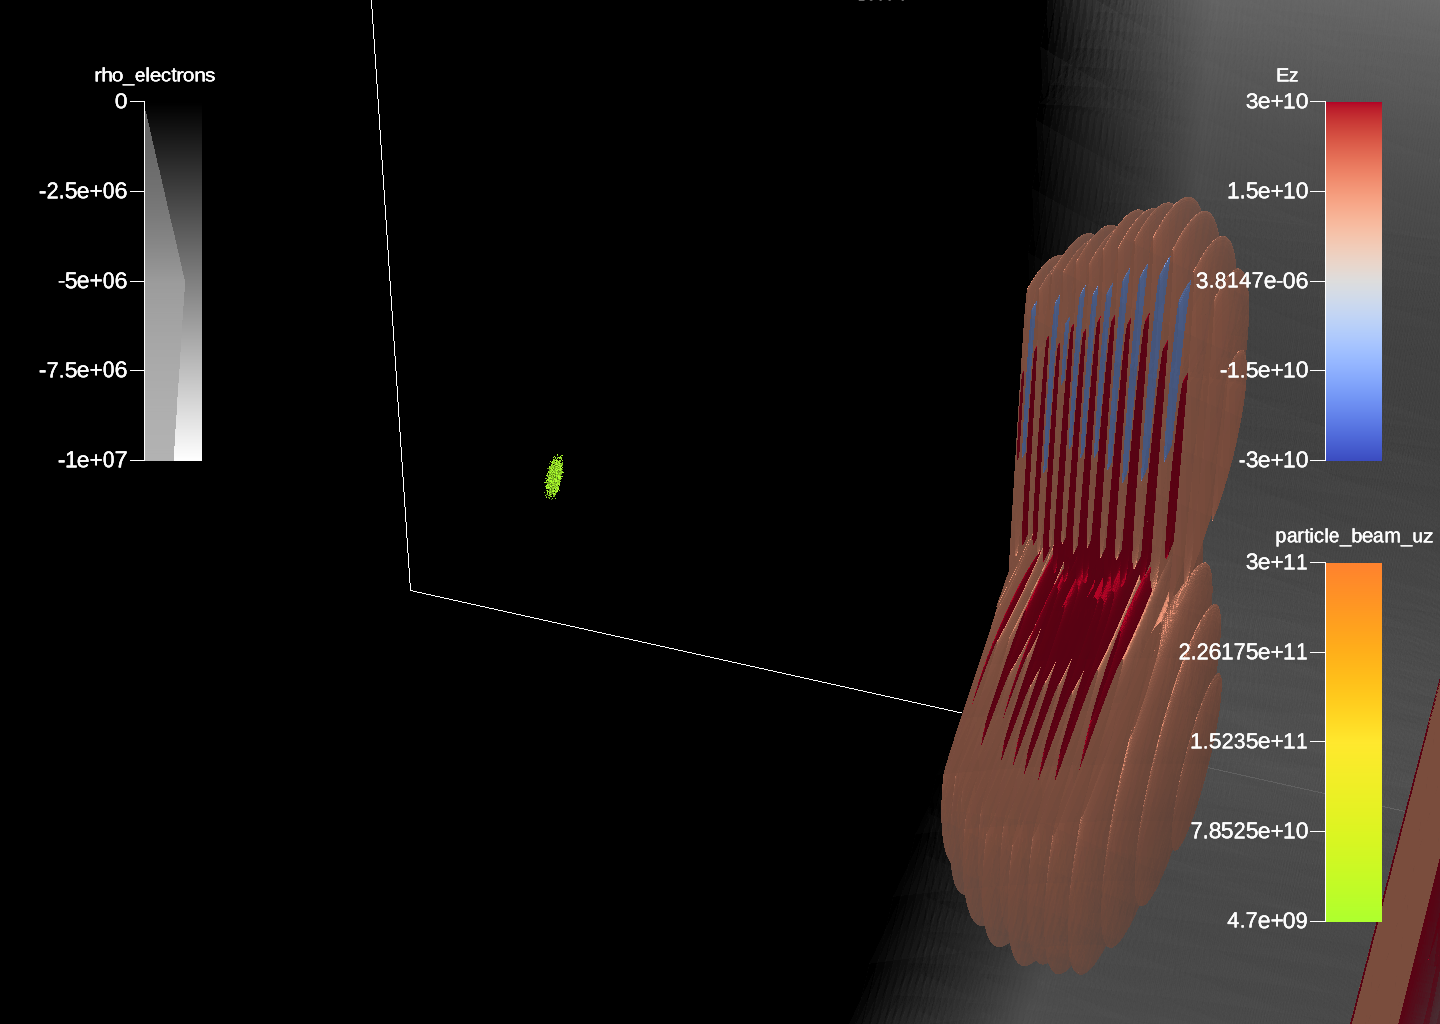
\includegraphics[width=0.475\textwidth]{ez_007050}
    & &
    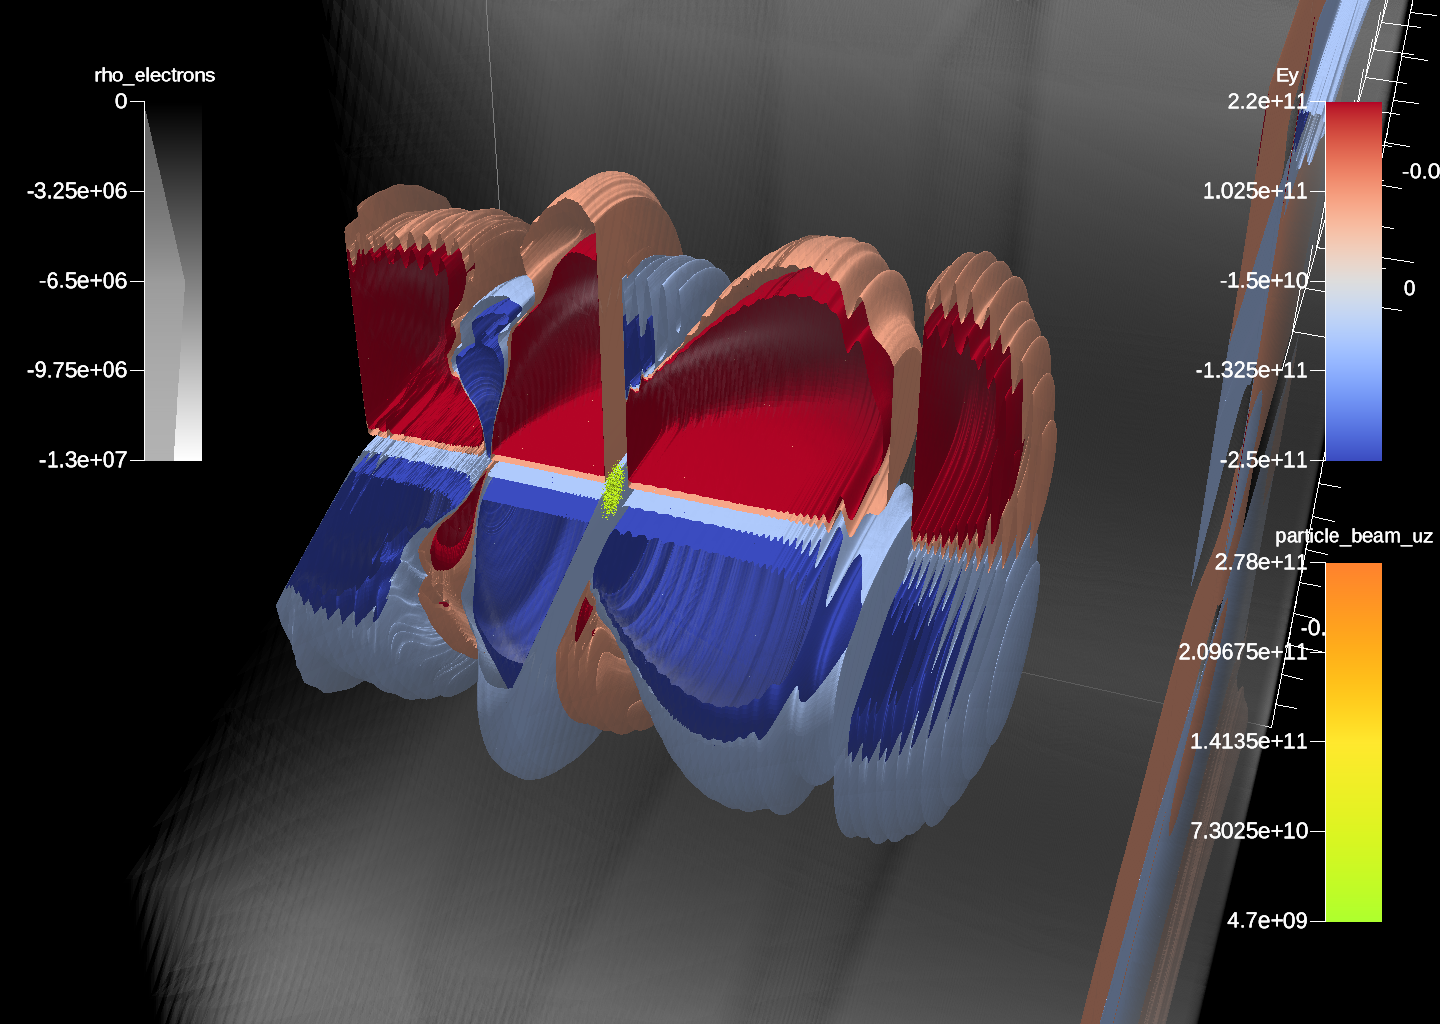
\includegraphics[width=0.475\textwidth]{ey_009300}
    \\
    \begin{minipage}{0.475\textwidth}
      \caption{
        WarpX in-situ visualization of a laser-wakefield accelerator on 4,416 GCDs across 552 nodes of Frontier using Ascent and \vtkm.
        The image depicts an early time step of the simulation at high resolution.
        \label{fig:warpx_highres}
      }
    \end{minipage}
    & &
    \begin{minipage}{0.475\textwidth}
      \caption{
        WarpX in-situ visualization of a laser-wakefield accelerator on 552 GCDs across 69 nodes of Frontier using Ascent and \vtkm.
        The image depicts a later time step of the simulation at low resolution.
        \label{fig:warpx_lowres}
      }
    \end{minipage}
  \end{tabularx}
\end{figure*}

\begin{figure*}[ht]
  \centering
  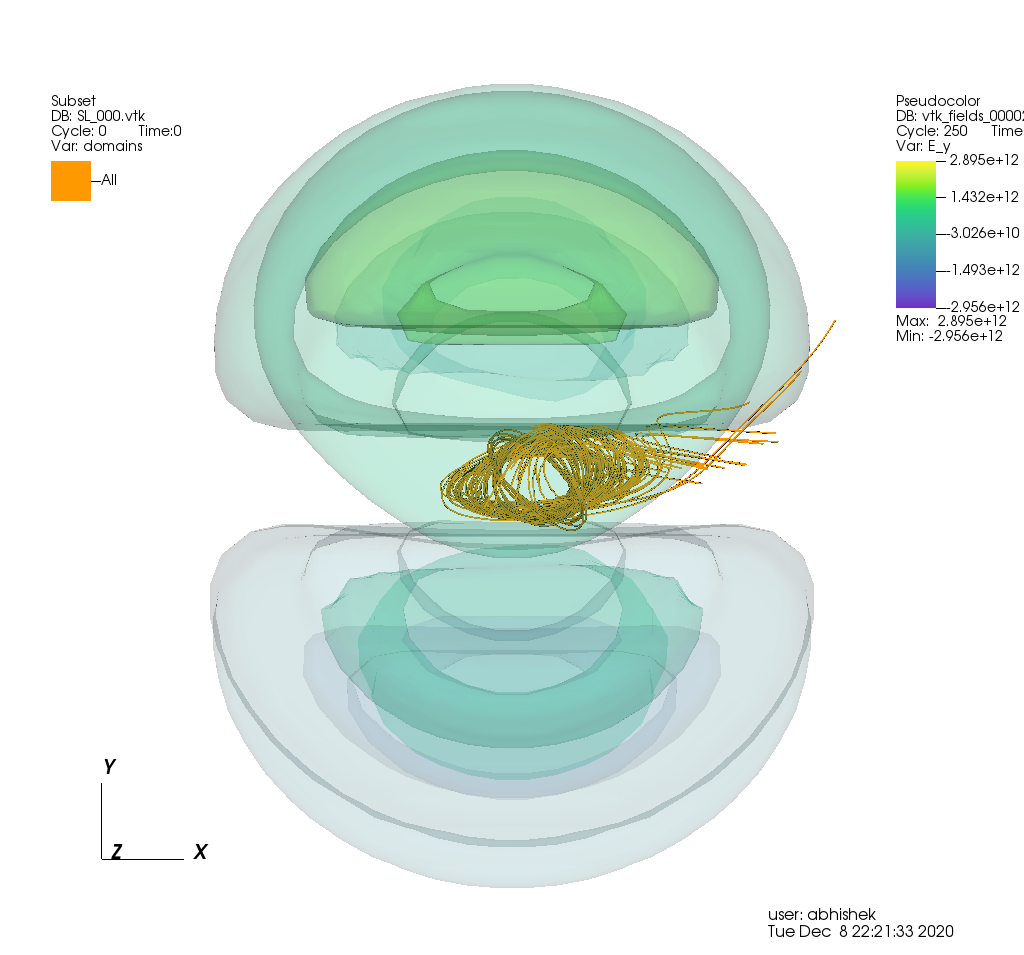
\includegraphics[width=0.49\linewidth]{lwfa_particle_advection_front}%
  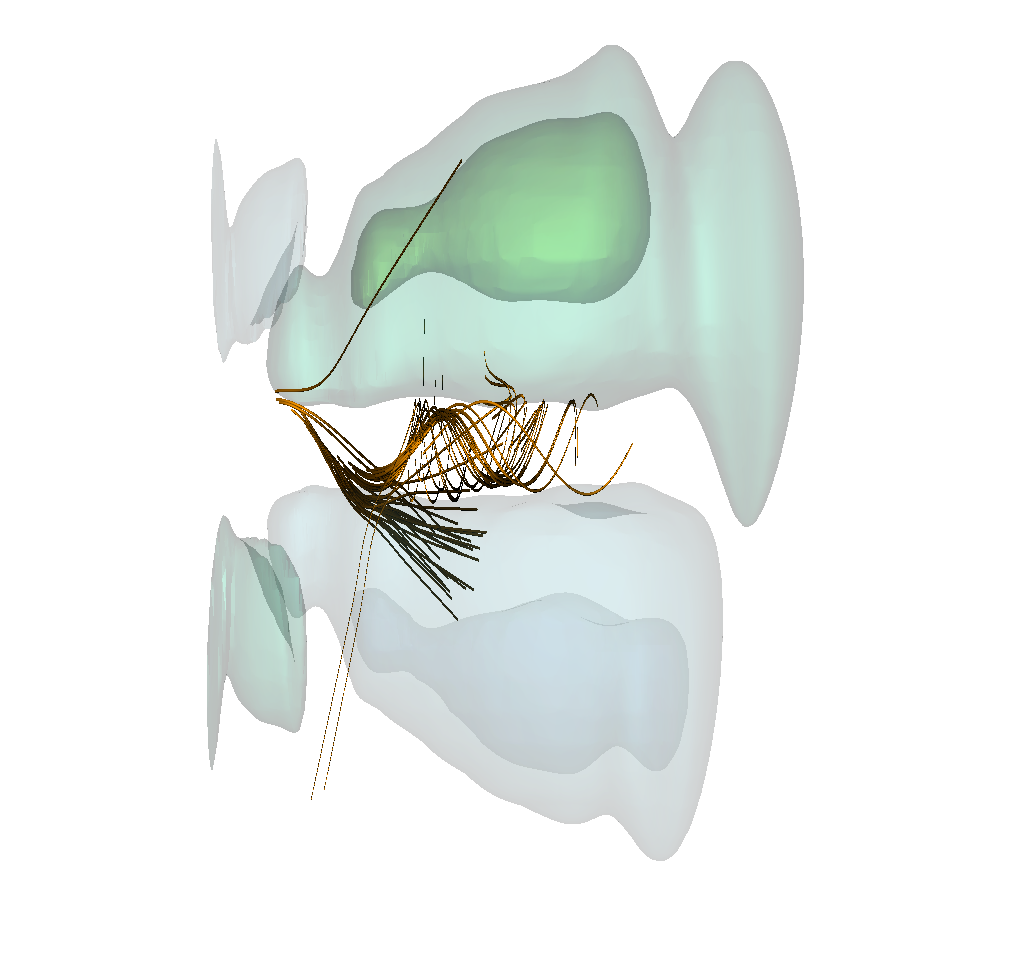
\includegraphics[width=0.49\linewidth]{lwfa_particle_advection_side}
  \caption{Side and front views of a laser wakefield with an injected electron bunch.
  Particles are advected from \emph{a single snapshot} of the simulation in \vtkm.}
  \label{fig:lwfa_particle_advection}
\end{figure*}

\subsection{Laser Wakefield Acceleration}\label{sec:warpx}

%\assign{Axel, Abhi}~%
%
%\defcitealias{FedeliHuebl2022}{Fedeli, Huebl et al. (2022)}
%\citepalias{FedeliHuebl2022}
%
WarpX is a particle-in-cell simulation code and was awarded the 2022 ACM Gordon Bell Prize~\citep{FedeliHuebl2022}.
As part of the ECP, WarpX was developed as a new application to succeed its predecessor, Warp~\citep{Vay2013}, with the goal of studying advanced particle acceleration in laser-driven plasma wakefields in an effort to advance future high-energy physics colliders~\citep{Albert2021}.
Beyond that, WarpX is used to describe kinetic physics in particle accelerators, laser-plasmas, fusion devices, inertial confinement fusion, and astrophysical plasmas and to model microelectronics~\citep{Yao2022}.

Figures \ref{fig:warpx_highres} and \ref{fig:warpx_lowres} are in-situ renderings of a \emph{staged} laser wakefield accelerator in a boosted reference frame~\citep{Vay2011}.
An electron beam (orange-green) is accelerated to the right through multiple stages to high energies.
In the plasma stages (gray), the strong traversal focusing fields are shown in red-blue.

In the staging approach, a particle beam is accelerated through multiple plasma elements.
In each stage, an ultra-intense laser pulse excites a plasma wakefield.
This depletes the laser pulse's energy and generates very strong electric fields in the plasma wake, which can be used to accelerate an injected electron beam.
The acceleration itself can be 3--4 orders of magnitude more compact than relying on state-of-the-art radio-frequency accelerator elements.
Besides increased beam energy, physicists study how to preserve beam properties essential for transport, focusing (e.g., emittance), and applications (e.g., charge and current).

WarpX features advanced techniques such as GPU-acceleration for three vendors, mesh-refinement capabilities, dynamic load balancing, and unique advanced numerical solvers.
WarpX relies on multi-level parallelization: coarse parallelization uses block-structured domain decomposition with MPI using the AMReX library~\citep{Zhang2019}, and compute acceleration leverages CUDA/HIP/SYCL or OpenMP so that the simulations can scale on large, massively parallel HPC systems.

% Included here to be close to next subsection.
\begin{figure*}[b]
  \centering
  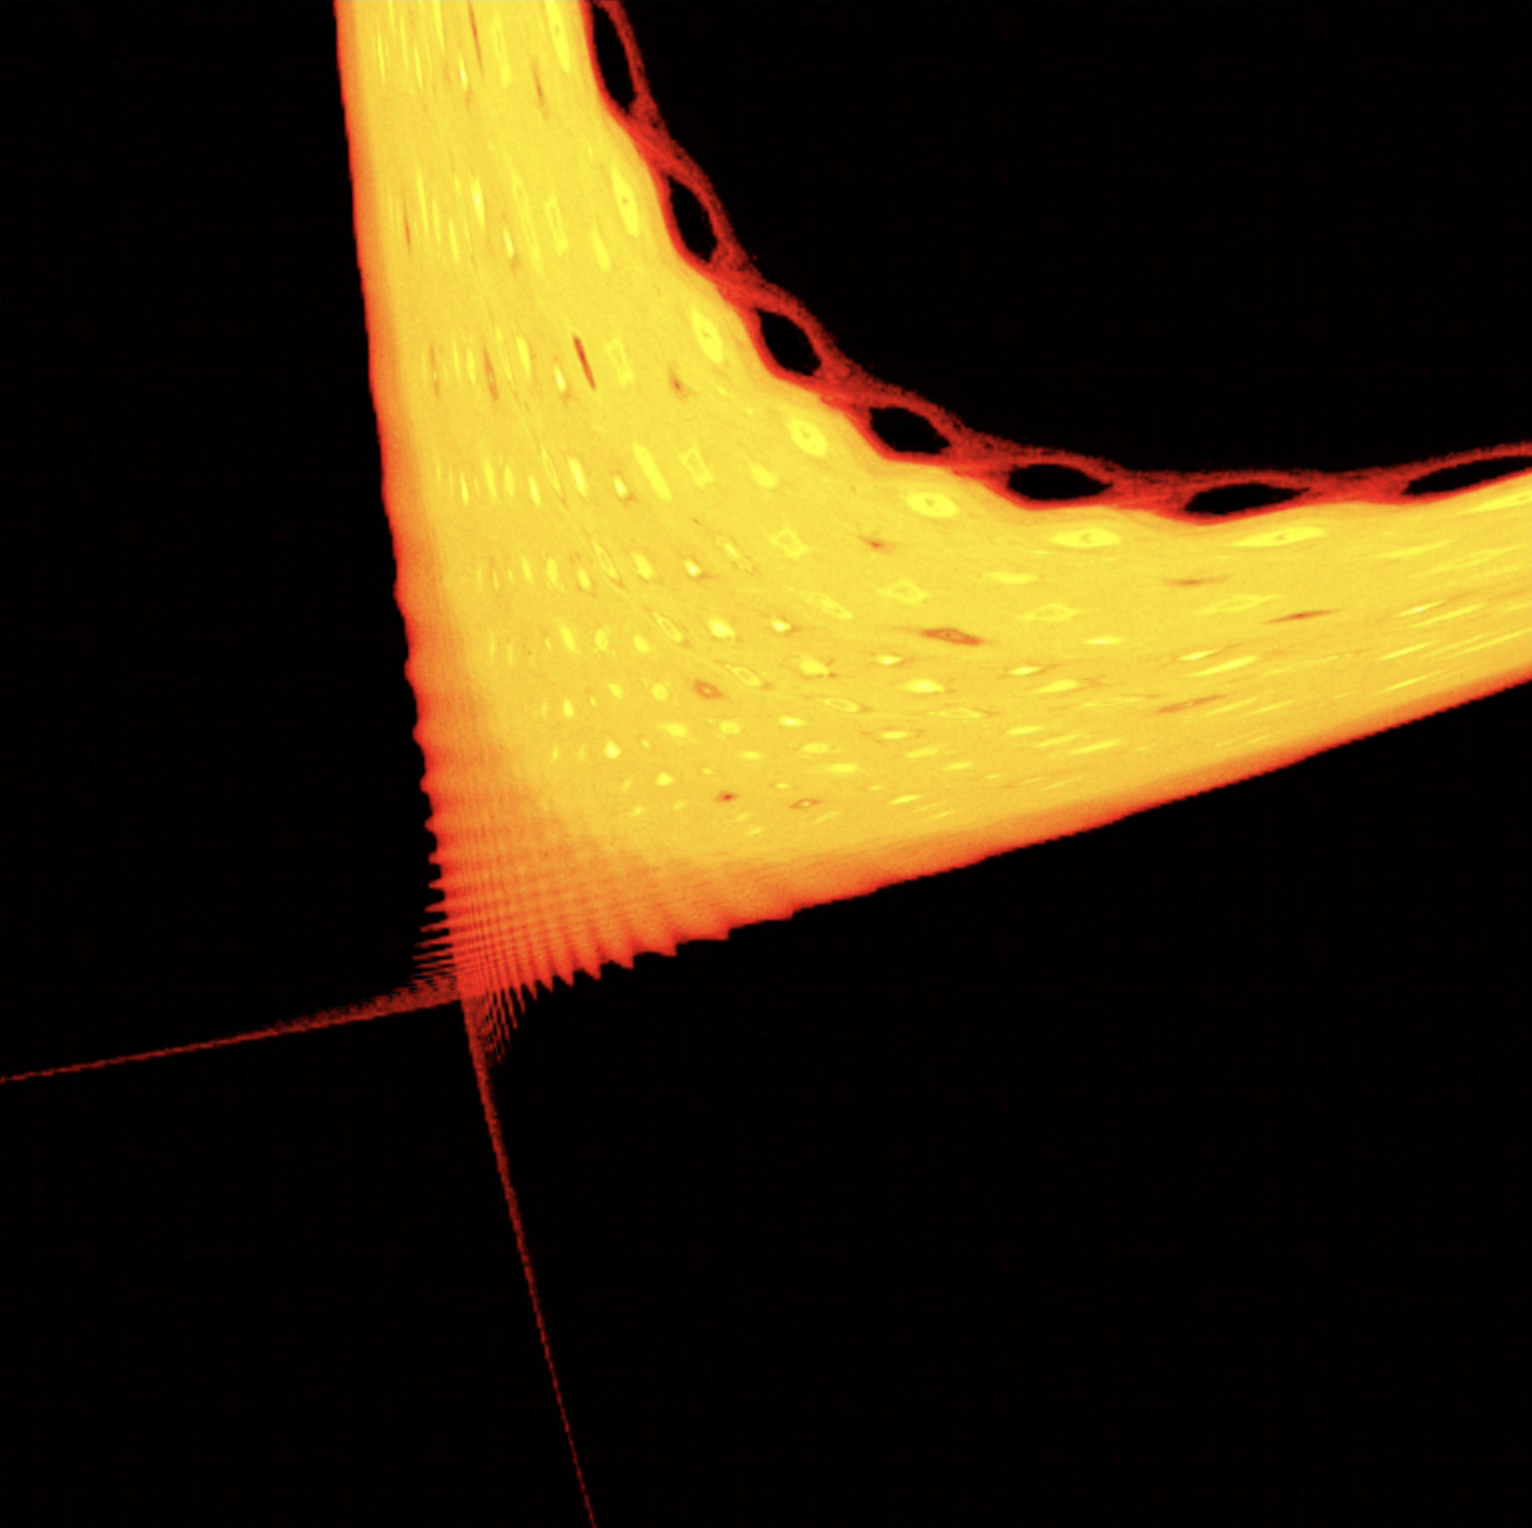
\includegraphics[width=0.49\linewidth]{poincare1}
  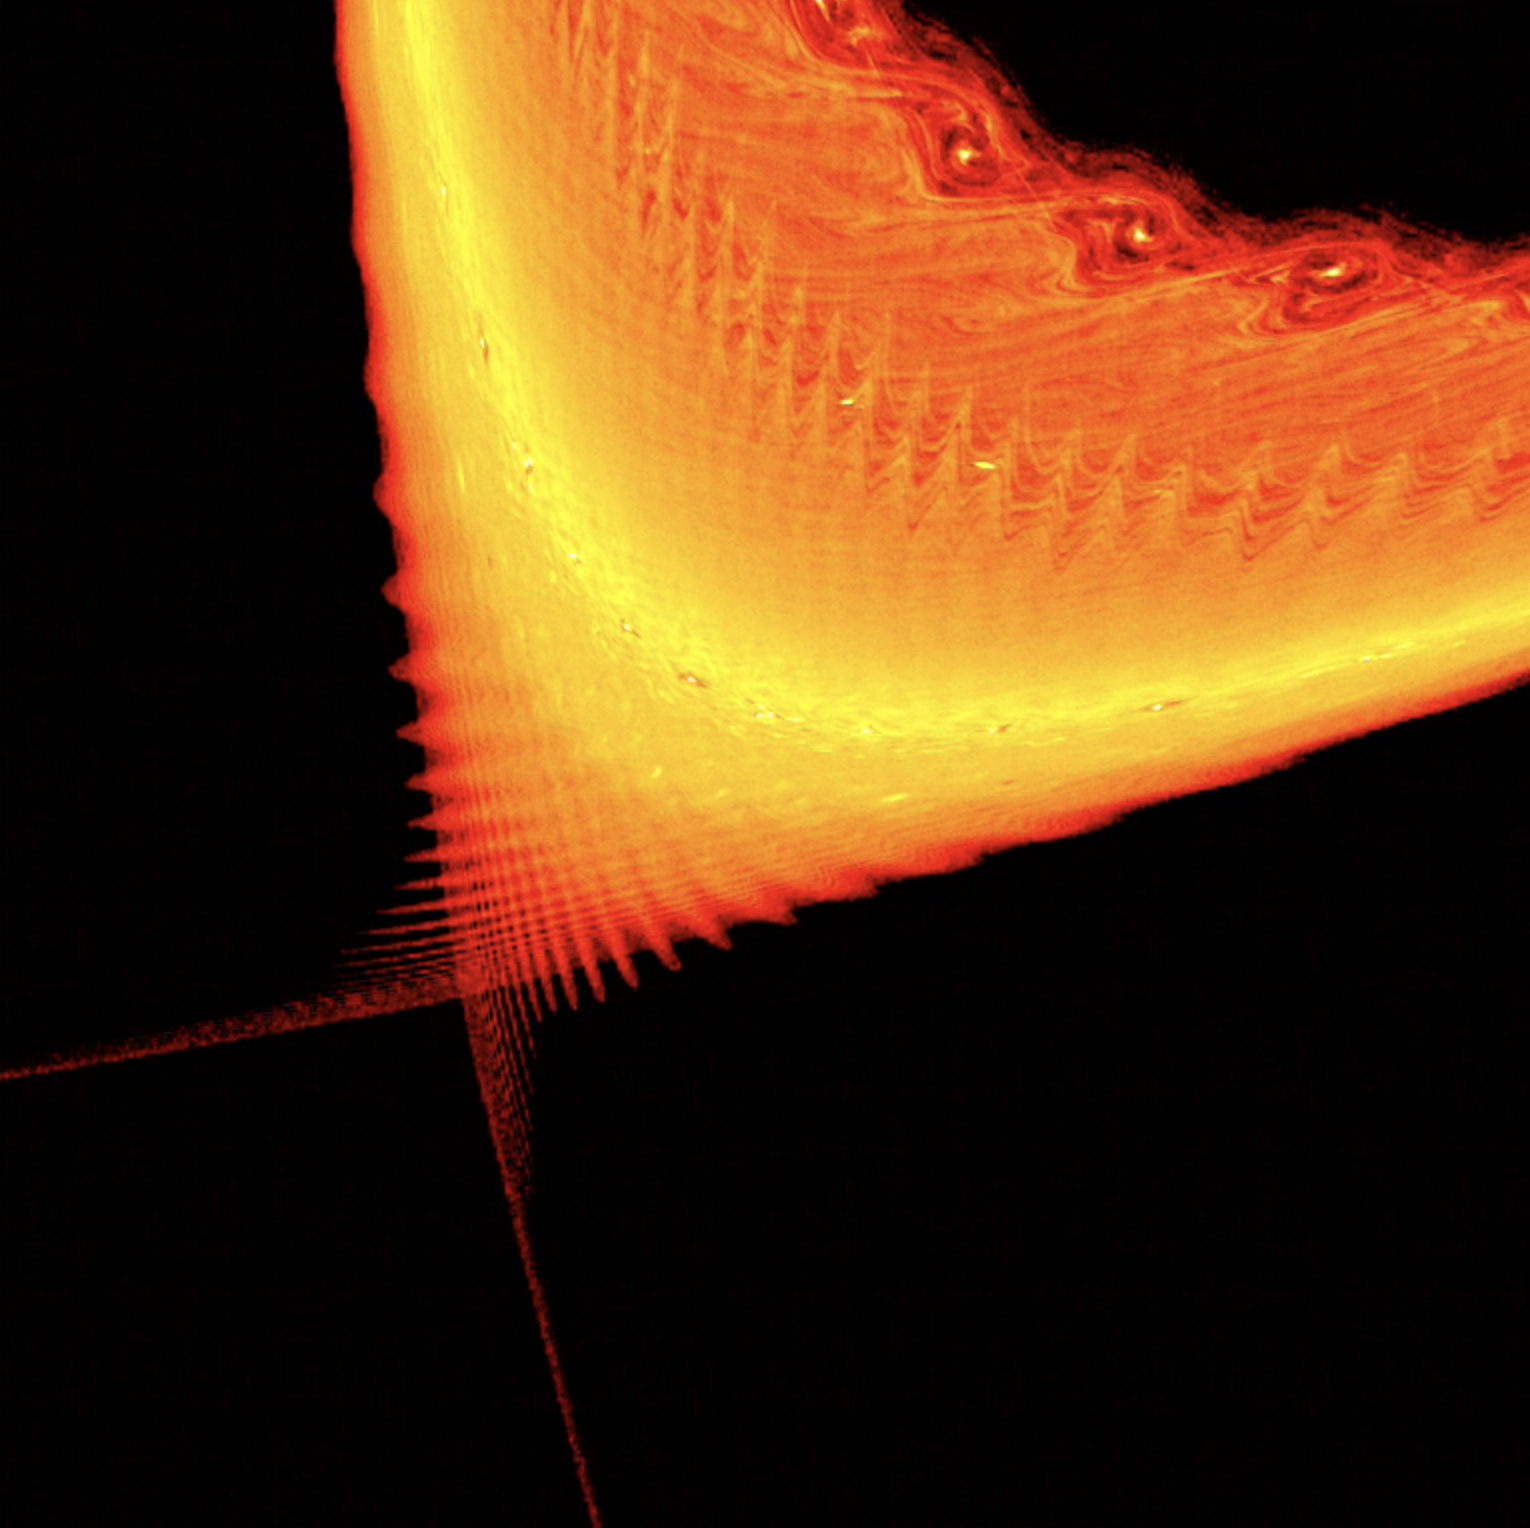
\includegraphics[width=0.49\linewidth]{poincare2}
  \caption{\poincare maps from two different time steps from a simulation run at the Oak Ridge Leadership Computing Facility generated by \vtkm.  The particles were placed near the edge of the tokamak where the plasma becomes very turbulent. The \poincare map shows magnetic features in the plasma as the simulation progresses. Of particular interest are the long fingers that appear in the lower portion of the image. The evolving shape of these fingers over time provides valuable insight into the behavior of the magnetic field where the turbulence is extremely high. }
  \label{fig:poincare}
\end{figure*}

If WarpX relied on only traditional post-processing workflows for the visualization of the dynamics of exascale simulations, the resulting multi-petabyte scale output per simulation would severely limit the available snapshots and/or level of detail to visualize.
Addressing this need, WarpX interfaces with Ascent for in-situ visualization.
For this, utility routines for specialized WarpX diagnostics for application-specific descriptions were implemented in AMReX.
WarpX performs data preparation steps for diagnostics in situ, shares the respective AMReX memory buffers with zero-copy APIs through Conduit with Ascent, and renders with \vtkm in the same domain-decomposition and on the same compute device as the simulation itself.

Realistic visualization of particle trajectories (advection) in a plasma or particle accelerator requires high temporal fidelity in traditional workflows, and this fidelity can create significant data overhead.
With \vtkm, an opportunity to significantly reduce data input for such workflows was identified by using a physics-motivated advection algorithm and the slowly changing nature of fields in a wakefield accelerator.

Plasma particles such as electrons and ions are inert and can be relativistic, which effectively changes their mass as they move.
Traditional advection algorithms only used local properties of fields without accounting for a history or inert nature of a streamline.
As in a particle-in-cell algorithm, the realistic track of a charged plasma particle can be integrated following the Lorentz-Force, which interpolates six local field components ($E_{x,y,z}, B_{x,y,z}$) and advances the particles' momentum (inertia) and position with an explicit iteration scheme~\citep{Boris1970}.
The updated momentum is tracked over the path of a streamline to account for the evolving particle.

With this advection algorithm integrated in \vtkm, a snapshot of a simulation can be used to project the particles' physical position forward (and backward) for a meaningful time under the realistic assumption that fields are quasi-static (i.e., do not change much in time) besides translation along an axis.
Figure~\ref{fig:lwfa_particle_advection} shows such particle trajectories of an off-axis injected electron beam in a wakefield calculated from a single snapshot and reproducing physical betatron oscillation.


\subsection{Tokamak Fusion Reactor}

%\assign{Dave}

Fusion energy research focuses on understanding the science needed to develop energy sources based on the controlled fusion of light atomic nuclei. One strategy to achieve fusion involves a device called a tokamak, which uses magnetic fields to confine a hot plasma in the shape of a torus.
Significant efforts are currently underway to prepare for ITER, a large experimental fusion reactor under construction in France.
The Whole Device Model Application (WDMApp) is a project in the ECP that aims to develop a high-fidelity model of magnetically confined fusion plasma in tokamaks. 
WDMApp is critical in the efforts to plan experiments on ITER and optimize the design of future next-step fusion facilities. These devices will operate in physics regimes not achieved by any current or past experiments, thereby making advanced and predictive numerical simulation the best tool for the task.


%WDMApp is focused on building the main driver and coupling framework for the more complete Whole Device Model (WDM), with the ultimate goal of completing a comprehensive computational suite that includes all the physics components required to simulate a magnetically confined fusion reactor. The main driver for the WDM will be the coupling of two advanced gyrokinetic codes, one in the edge (XGC~\citep{XGC}) and the other in the core (GENE~\citep{GENE} or GEM~\citep{GEM}). XGC is a particle-in-cell (PIC) code optimized for treating the edge plasma. While GENE is a continuum code, GEM is a PIC code optimized for the core plasma. WDMApp takes advantage of the complementary nature of these two applications in the core to build the most advanced and efficient whole-device kinetic transport kernel for the WDM, and also to mitigate risk.


The behavior and evolution of the magnetic field in a tokamak is complex, and its control is critical for performance.
For these reasons, analysis tools used for understanding the dynamic nature of the magnetic field are critical.
The complexity of the 3D magnetic field lines makes analysis and visualization difficult.
Because the field lines are periodic, this complexity can be reduced by using a \poincare magnetic field-line puncture map~\citep{Sanderson2010}. 
The \poincare map is the intersection of a field line with a lower-dimensional subspace (called the \poincare section).
In our case, the \poincare section is a 2D plane that is perpendicular to the axis of the tokamak.
Given a set of magnetic field lines, the \poincare map (i.e., the intersection of the magnetic field lines with the plane) provides a concise 
representation of the magnetic field and is easier to understand and analyze.
Figure~\ref{fig:poincare} shows some examples of \poincare plots generated by \vtkm.

In practice, the \poincare map is generated by creating many field lines and plotting each intersection, or puncture, with the plane.
After a sufficient number of punctures has been collected, patterns in the map characterize the features in the magnetic field.
The field lines are computed by modeling massless particles that follow magnetic field lines.
These massless particles can follow magnetic field lines by advecting them in the direction of the magnetic field.
The intersections generated from a single particle characterize the features of the magnetic surface at that position.
The particles are advected using a differential equation solver such as the fourth order Runge-Kutta scheme.

Proper characterization of the magnetic field requires a large number of initial positions (typically tens of thousands), each of which typically results in between 1,000 and 3,000 intersections, with each intersection following a field line all the way through the tokamak's torus.
Because of these numerous features, the computation of a \poincare map can be very expensive.
The WDMApp team has a \poincare map code that runs on CPUs and takes several hours for the largest analysis run. 
%Because of this cost, the generation \poincare maps required careful planning.
The high cost of the analysis is due to two main factors: (1) the many particles and intersections required and (2) the complexity of the magnetic field calculation.  In many applications of particle advection, the vector field is calculated at the nodes of each cell in the mesh. Linear interpolation within the cell is used to evaluate the magnetic field for the particle being advected. Because of the large number of advection steps required for each particle in the \poincare map, small errors can rapidly accumulate. These errors are compounded because the evaluation of the magnetic field requires a complex set of calculations, and these calculations require high-order interpolation of several quantities.

Using \vtkm can significantly accelerate the computation of \poincare maps by leveraging the parallelism of GPUs. Because the trajectory of each particle is completely independent, the task can be parallelized over each particle. Using this approach, a \poincare map can be computed in under $3$ minutes. The wall-clock time for a typical WDMApp simulation step is between $1.5$ and $2$ minutes, which means that \poincare maps can be computed in situ in nearly real time.
When WDMApp is run, the EFFIS workflow control system~\citep{Suchyta2022:effis} allocates an additional 1--2 nodes for the \poincare map analysis. As a simulation step completes, EFFIS launches a \poincare analysis task on GPUs in the node in a round-robin fashion. This allows asynchronous analysis to be performed on the additional nodes while the simulation is running.
Because EFFIS was already being used as a code-integrating technology, it was straightforward to integrate \vtkm directly into this system.
Figure~\ref{fig:poincare} shows \poincare maps from two different time steps of a simulation run at the OLCF.
Real-time generation of \poincare maps provides the WDMApp team with unprecedented capability for analysis of magnetic fields in fusion simulations.


\subsection{Impact Beyond ECP}

%\assign{Jay}

%\jay{discuss the applications/use cases outside of ECP}
In addition to the applications mentioned above, \vtkm still serves as the key infrastructure for accelerating data analysis and visualization in various scientific applications through in-situ visualization. This subsection lists several examples and illustrates how \vtkm is integrated into in-situ scientific workflows outside of the ECP.


\begin{figure}[htb]
  \centering
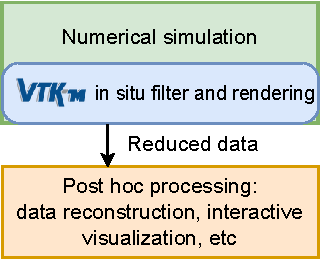
\includegraphics[width=0.60\linewidth]{vtkm_insitu_posthoc}
\caption{The in-situ reduction + post-hoc paradigm based on \vtkm.}
\label{fig:vtkm_insitu_posthoc}
\end{figure}

Before being selected as a project in the ECP, \vtkm was a core component in the Visualization for the Extreme-Scale Scientific Computation Ecosystem (XVis)~\citep{Moreland2019} project. 
XVis focused on multiple ways to integrate in-situ visualization with the simulation, extract key information, and decrease the data size for post-hoc processing.
The \textit{in-situ reduction + post hoc} paradigm (Figure~\ref{fig:vtkm_insitu_posthoc}) is adopted in multiple scientific domains within and outside of the ECP, such as probability distribution function extraction of fields in combustion simulation~\citep{Ye2016} and binning mechanisms to reduce the data size of fusion simulation~\citep{Kress2018}. We use two recent efforts as examples to illustrate how \vtkm facilitates scientific workflows beyond the ECP.


Nyx is a cosmological simulation code that aims to solve compressible hydrodynamics with $N$-body treatment of dark matter. Each simulation run may contain hundreds of time steps with multiple sets of simulation input parameters. The raw data size is usually hundreds of terabytes to several petabytes---a size that presents challenges when post-processing the data. 
\vtkm is used for in-situ analysis to extract the statistical properties of the down-sampled data to significantly reduce the size of raw data. The associated statistics model can be used to construct the data based on prior knowledge in post-processing with low data reconstruction error~\citep{Wang2019}.

Eddy detection and tracking play key roles in analyzing the data generated by ocean simulations. Understanding the characteristics of eddies can help scientists explain the regional air-sea interactions.
The \vtkm streamline filter can be used as an in-situ analysis to generate streamline data used for interactive post-hoc analysis~\citep{Han2022}. With the help of \vtkm, the associated eddy analysis workflow can improve the interaction speed, reduce data storage, and meet the
needs of real-time visual analysis interaction.  

% TODO, add a summary figure, altough not use ECP solution, vtk-m play key role in developing insitu solution

\section{Conclusion}

%\assign{Ken}

GPUs and other accelerators have become a staple of HPC.
Although they were anomalous a decade ago, GPUs are now featured on over $1/3$ of the top 500 fastest supercomputers,\footnote{\url{https://top500.org/lists/top500/2023/11/}} and that number is rising.
Efficient use of these accelerators is critical for good performance on HPC systems, and \vtkm provides this functionality for scientific visualization.

ECP has been instrumental in making \vtkm available on today's Exascale machines.
Many challenges were overcome with porting and integrating the software, and we are proud to have helped application scientists analyze, explore, and understand their data.
We anticipate the use of \vtkm in high performance visualization software to be even more critical as HPC machines evolve.

\section{Acknowledgments}

%\assign{Hank, make a nice statement about contributors.}

The work in this paper builds upon a foundation laid by many previous members of the \vtkm team as well as early adopters.  We thank and acknowledge
Cyrus Harrison, 
Nrushad Joshi,
Brad King, 
Matthew Larsen,
Robert Maynard, 
Jeremy Meredith, 
Chris Sewell,
and
Allison Vacanti.
%Axel Huebl acknowledges
The authors also acknowledge
the WarpX and AMReX open-source community members and WarpX PI Jean-Luc Vay
for their roles in integrating \vtkm and WarpX technologies.
%\ken{Would it read better to replace ``Axel Huebl acknowledges'' with ``We thank and acknowledge''?}

This research was supported by the ECP (17-SC-20-SC), a collaborative effort of the DOE's Office of Science and the National Nuclear Security Administration.
This research used resources of the OLCF at ORNL, which is supported by the DOE's Office of Science under contract number DE-AC05-00OR22725.
This research also used resources of the ALCF, a DOE Office of Science user facility at Argonne National Laboratory and is based on research supported by the DOE Office of Science-Advanced Scientific Computing Research Program under contract number DE-AC02-06CH11357. This work was conducted on a preproduction supercomputer with early versions of the Aurora software development kit.


\bibliographystyle{SageH}
\bibliography{IJHPCASpecialIssue_VTKm}

\end{document}

\iffalse
% sage_latex_guidelines.tex V1.20, 14 January 2017

\documentclass[Afour,sageh,times]{sagej}

\usepackage{moreverb,url}

\usepackage[colorlinks,bookmarksopen,bookmarksnumbered,citecolor=red,urlcolor=red]{hyperref}

\newcommand\BibTeX{{\rmfamily B\kern-.05em \textsc{i\kern-.025em b}\kern-.08em
T\kern-.1667em\lower.7ex\hbox{E}\kern-.125emX}}

\def\volumeyear{2016}

\begin{document}

\runninghead{Smith and Wittkopf}

\title{A demonstration of the \LaTeXe\ class file for
\itshape{SAGE Publications}}

\author{Alistair Smith\affilnum{1} and Hendrik Wittkopf\affilnum{2}}

\affiliation{\affilnum{1}Sunrise Setting Ltd, UK\\
\affilnum{2}SAGE Publications Ltd, UK}

\corrauth{Alistair Smith, Sunrise Setting Ltd
Brixham Laboratory,
Freshwater Quarry,
Brixham, Devon,
TQ5~8BA, UK.}

\email{alistair.smith@sunrise-setting.co.uk}

\begin{abstract}
This paper describes the use of the \LaTeXe\
\textsf{\journalclass} class file for setting papers to be
submitted to a \textit{SAGE Publications} journal.
The template can be downloaded \href{http://www.uk.sagepub.com/repository/binaries/SAGE LaTeX template.zip}{here}.
\end{abstract}

\keywords{Class file, \LaTeXe, \textit{SAGE Publications}}

\maketitle

\section{Introduction}
Many authors submitting to research journals use \LaTeXe\ to
prepare their papers. This paper describes the
\textsf{\journalclass} class file which can be used to convert
articles produced with other \LaTeXe\ class files into the correct
form for submission to \textit{SAGE Publications}.

The \textsf{\journalclass} class file preserves much of the
standard \LaTeXe\ interface so that any document which was
produced using the standard \LaTeXe\ \textsf{article} style can
easily be converted to work with the \textsf{\journalclassshort}
style. However, the width of text and typesize will vary from that
of \textsf{article.cls}; therefore, \textit{line breaks will change}
and it is likely that displayed mathematics and tabular material
will need re-setting.

In the following sections we describe how to lay out your code to
use \textsf{\journalclass} to reproduce much of the typographical look of
the \textit{SAGE} journal that you wish to submit to. However, this paper is not a guide to
using \LaTeXe\ and we would refer you to any of the many books
available (see, for example, \cite{R1}, \cite{R2} and \cite{R3}).

\section{The three golden rules}
Before we proceed, we would like to stress \textit{three golden
rules} that need to be followed to enable the most efficient use
of your code at the typesetting stage:
\begin{enumerate}
\item[(i)] keep your own macros to an absolute minimum;

\item[(ii)] as \TeX\ is designed to make sensible spacing
decisions by itself, do \textit{not} use explicit horizontal or
vertical spacing commands, except in a few accepted (mostly
mathematical) situations, such as \verb"\," before a
differential~d, or \verb"\quad" to separate an equation from its
qualifier;

\item[(iii)] follow the journal reference style.
\end{enumerate}

\section{Getting started} The \textsf{\journalclassshort} class file should run
on any standard \LaTeXe\ installation. If any of the fonts, style
files or packages it requires are missing from your installation,
they can be found on the \textit{\TeX\ Collection} DVDs or downloaded from
CTAN.

\begin{figure*}
\setlength{\fboxsep}{0pt}%
\setlength{\fboxrule}{0pt}%
\begin{center}
\begin{boxedverbatim}
\documentclass[<options>]{sagej}

\begin{document}

\runninghead{<Author surnames>}

\title{<Initial capital only>}

\author{<An Author\affilnum{1},
Someone Else\affilnum{2} and
Perhaps Another\affilnum{1}>}

\affiliation{<\affilnum{1}First and third authors' affiliation\\
\affilnum{2}Second author affiliation>}

\corrauth{<Corresponding author's name and full postal address>}

\email{<Corresponding author's email address>}

\begin{abstract}
<Text>
\end{abstract}

\keywords{<List keywords>}

\maketitle

\section{Introduction}
.
.
.
\end{boxedverbatim}
\end{center}
\caption{Example header text.\label{F1}}
\end{figure*}

\section{The article header information}
The heading for any file using \textsf{\journalclass} is shown in
Figure~\ref{F1}. You must select options for the trim/text area and
the reference style of the journal you are submitting to.
The choice of \verb+options+ are listed in Table~\ref{T1}.

\begin{table}[h]
\small\sf\centering
\caption{The choice of options.\label{T1}}
\begin{tabular}{lll}
\toprule
Option&Trim and font size&Columns\\
\midrule
\texttt{shortAfour}& 210 $\times$ 280 mm, 10pt& Double column\\
\texttt{Afour} &210 $\times$ 297 mm, 10pt& Double column\\
\texttt{MCfour} &189 $\times$ 246 mm, 10pt& Double column\\
\texttt{PCfour} &170 $\times$ 242 mm, 10pt& Double column\\
\texttt{Royal} &156 $\times$ 234 mm, 10pt& Single column\\
\texttt{Crown} &7.25 $\times$ 9.5 in, 10pt&Single column\\
\texttt{Review} & 156 $\times$ 234 mm, 12pt & Single column\\
\bottomrule
\end{tabular}\\[10pt]
\begin{tabular}{ll}
\toprule
Option&Reference style\\
\midrule
\texttt{sageh}&SAGE Harvard style (author-year)\\
\texttt{sagev}&SAGE Vancouver style (superscript numbers)\\
\texttt{sageapa}&APA style (author-year)\\
\bottomrule
\end{tabular}
\end{table}

For example, if your journal is short A4 sized, uses Times fonts and has Harvard style references then you would need\\
{\small\verb+\documentclass[ShortAfour,times,sageh]{sagej}+}

Most \textit{SAGE} journals are published using Times fonts but if for any reason you have a problem using Times you can
easily resort to Computer Modern fonts by removing the
\verb"times" option.

\subsection{`Review' option}
Some journals (for example, \emph{Journal of the Society for Clinical Trials}) require that
papers are set single column and with a larger font size to help with the review process.
If this is a requirement for the journal that you are submitting to, just add the \verb+Review+ option to the \verb+\documenclass[]{sagej}+ line.

\subsection{Remarks}
\begin{enumerate}
\item[(i)] In \verb"\runninghead" use `\textit{et~al.}' if there
are three or more authors.

\item[(ii)] For multiple author papers please note the use of \verb"\affilnum" to
link names and affiliations. The corresponding author details need to be included using the
\verb+\corrauth+ and \verb+\email+ commands.

\item[(iii)] For submitting a double-spaced manuscript, add
\verb"doublespace" as an option to the documentclass line.

\item[(iv)] The abstract should be capable of standing by itself,
in the absence of the body of the article and of the bibliography.
Therefore, it must not contain any reference citations.

\item[(v)] Keywords are separated by commas.

\item[(vi)] If you are submitting to a \textit{SAGE} journal that requires numbered sections (for example, IJRR), please add the command
  \verb+\setcounter{secnumdepth}{3}+ just above the \verb+\begin{document}+ line.

\end{enumerate}


\section{The body of the article}

\subsection{Mathematics} \textsf{\journalclass} makes the full
functionality of \AmS\/\TeX\ available. We encourage the use of
the \verb"align", \verb"gather" and \verb"multline" environments
for displayed mathematics. \textsf{amsthm} is used for setting
theorem-like and proof environments. The usual \verb"\newtheorem"
command needs to be used to set up the environments for your
particular document.

\subsection{Figures and tables} \textsf{\journalclass} includes the
\textsf{graphicx} package for handling figures.

Figures are called in as follows:
\begin{verbatim}
\begin{figure}
\centering
\includegraphics{<figure name>}
\caption{<Figure caption>}
\end{figure}
\end{verbatim}

For further details on how to size figures, etc., with the
\textsf{graphicx} package see, for example, \cite{R1}
or \cite{R3}.

The standard coding for a table is shown in Figure~\ref{F2}.

\begin{figure}
\setlength{\fboxsep}{0pt}%
\setlength{\fboxrule}{0pt}%
\begin{center}
\begin{boxedverbatim}
\begin{table}
\small\sf\centering
\caption{<Table caption.>}
\begin{tabular}{<table alignment>}
\toprule
<column headings>\\
\midrule
<table entries
(separated by & as usual)>\\
<table entries>\\
.
.
.\\
\bottomrule
\end{tabular}
\end{table}
\end{boxedverbatim}
\end{center}
\caption{Example table layout.\label{F2}}
\end{figure}

\subsection{Cross-referencing}
The use of the \LaTeX\ cross-reference system
for figures, tables, equations, etc., is encouraged
(using \verb"\ref{<name>}" and \verb"\label{<name>}").

\subsection{End of paper special sections}
Depending on the requirements of the journal that you are submitting to,
there are macros defined to typeset various special sections.

The commands available are:
\begin{verbatim}
\begin{acks}
To typeset an
  "Acknowledgements" section.
\end{acks}
\end{verbatim}

\begin{verbatim}
\begin{biog}
To typeset an
  "Author biography" section.
\end{biog}
\end{verbatim}

\begin{verbatim}
\begin{biogs}
To typeset an
  "Author Biographies" section.
\end{biogs}
\end{verbatim}

%\newpage

\begin{verbatim}
\begin{dci}
To typeset a "Declaration of
  conflicting interests" section.
\end{dci}
\end{verbatim}

\begin{verbatim}
\begin{funding}
To typeset a "Funding" section.
\end{funding}
\end{verbatim}

\begin{verbatim}
\begin{sm}
To typeset a
  "Supplemental material" section.
\end{sm}
\end{verbatim}

\subsection{Endnotes}
Most \textit{SAGE} journals use endnotes rather than footnotes, so any notes should be coded as \verb+\endnote{<Text>}+.
Place the command \verb+\theendnotes+ just above the Reference section to typeset the endnotes.

To avoid any confusion for papers that use Vancouver style references,  footnotes/endnotes should be edited into the text.

\subsection{References}
Please note that the files \textsf{SageH.bst} and \textsf{SageV.bst} are included with the class file
for those authors using \BibTeX.
The files work in a completely standard way, and you just need to uncomment one of the lines in the below example depending on what style you require:
\begin{verbatim}
%%Harvard (name/date)
%\bibliographystyle{SageH}
%%Vancouver (numbered)
%\bibliographystyle{SageV}
\bibliography{<YourBibfile.bib>}
\end{verbatim}
and remember to add the relevant option to the \verb+\documentclass[]{sagej}+ line as listed in Table~\ref{T1}. 

%\section{Support for \textsf{\journalclass}}
%We offer on-line support to participating authors. Please contact
%us via e-mail at \dots
%
%We would welcome any feedback, positive or otherwise, on your
%experiences of using \textsf{\journalclass}.

\section{Copyright statement}
Please  be  aware that the use of  this \LaTeXe\ class file is
governed by the following conditions.

\subsection{Copyright}
Copyright \copyright\ \volumeyear\ SAGE Publications Ltd,
1 Oliver's Yard, 55 City Road, London, EC1Y~1SP, UK. All
rights reserved.

\subsection{Rules of use}
This class file is made available for use by authors who wish to
prepare an article for publication in a \textit{SAGE Publications} journal.
The user may not exploit any
part of the class file commercially.

This class file is provided on an \textit{as is}  basis, without
warranties of any kind, either express or implied, including but
not limited to warranties of title, or implied  warranties of
merchantablility or fitness for a particular purpose. There will
be no duty on the author[s] of the software or SAGE Publications Ltd
to correct any errors or defects in the software. Any
statutory  rights you may have remain unaffected by your
acceptance of these rules of use.

\begin{acks}
This class file was developed by Sunrise Setting Ltd,
Brixham, Devon, UK.\\
Website: \url{http://www.sunrise-setting.co.uk}
\end{acks}

\begin{thebibliography}{99}
\bibitem[Kopka and Daly(2003)]{R1}
Kopka~H and Daly~PW (2003) \textit{A Guide to \LaTeX}, 4th~edn.
Addison-Wesley.

\bibitem[Lamport(1994)]{R2}
Lamport~L (1994) \textit{\LaTeX: a Document Preparation System},
2nd~edn. Addison-Wesley.

\bibitem[Mittelbach and Goossens(2004)]{R3}
Mittelbach~F and Goossens~M (2004) \textit{The \LaTeX\ Companion},
2nd~edn. Addison-Wesley.

\end{thebibliography}

\end{document}
\fi
